%   Filename    : chapter_4.tex 
\chapter{Results and Discussion}
This chapter presents the results of the study, specifically TUKIB's various interfaces and pages, features, and backend implementation. As such, the figures shown herein are screenshots of TUKIB.

\section{User Interface}

\subsection{Landing Page}

\figref{fig:landing} showcases the landing page of the website for the system. The page features easy navigation to essential information and pages including home, news and announcements, services, laboratories, and about. A log in button is also included on the top right of the page to ensure that user's can quickly access their accounts. Additionally, a persistent button for the chatbot is found on the bottom left of the page. 

\begin{figure}[h]
	\centering 
	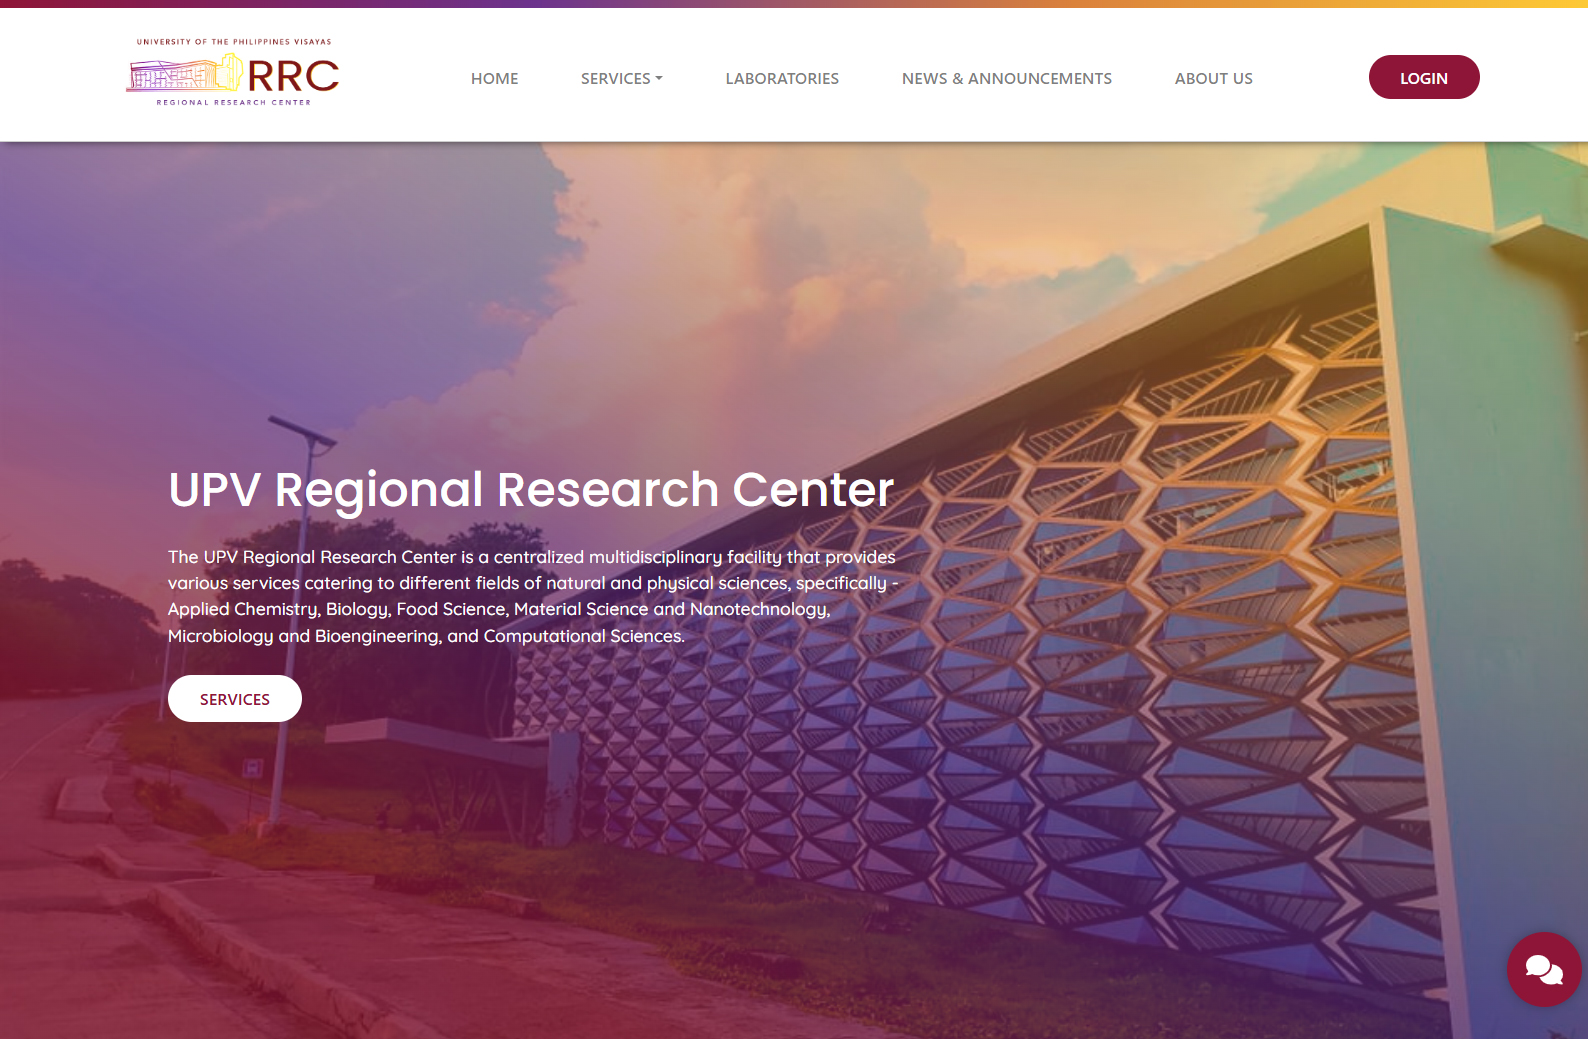
\includegraphics[width=0.75\textwidth]{landing.png}
	\caption{Landing/Homepage}
	\label{fig:landing}
\end{figure}

\subsection{Services Page}

Figure \ref{fig:service_page} shows the `Services' page. Each service has a separate page that includes a description of the service, pricing information, and instructions or guide on how to avail the service. This structure facilitates easier navigation and helps users find the information they need efficiently.

\begin{figure}[h]
	\centering
	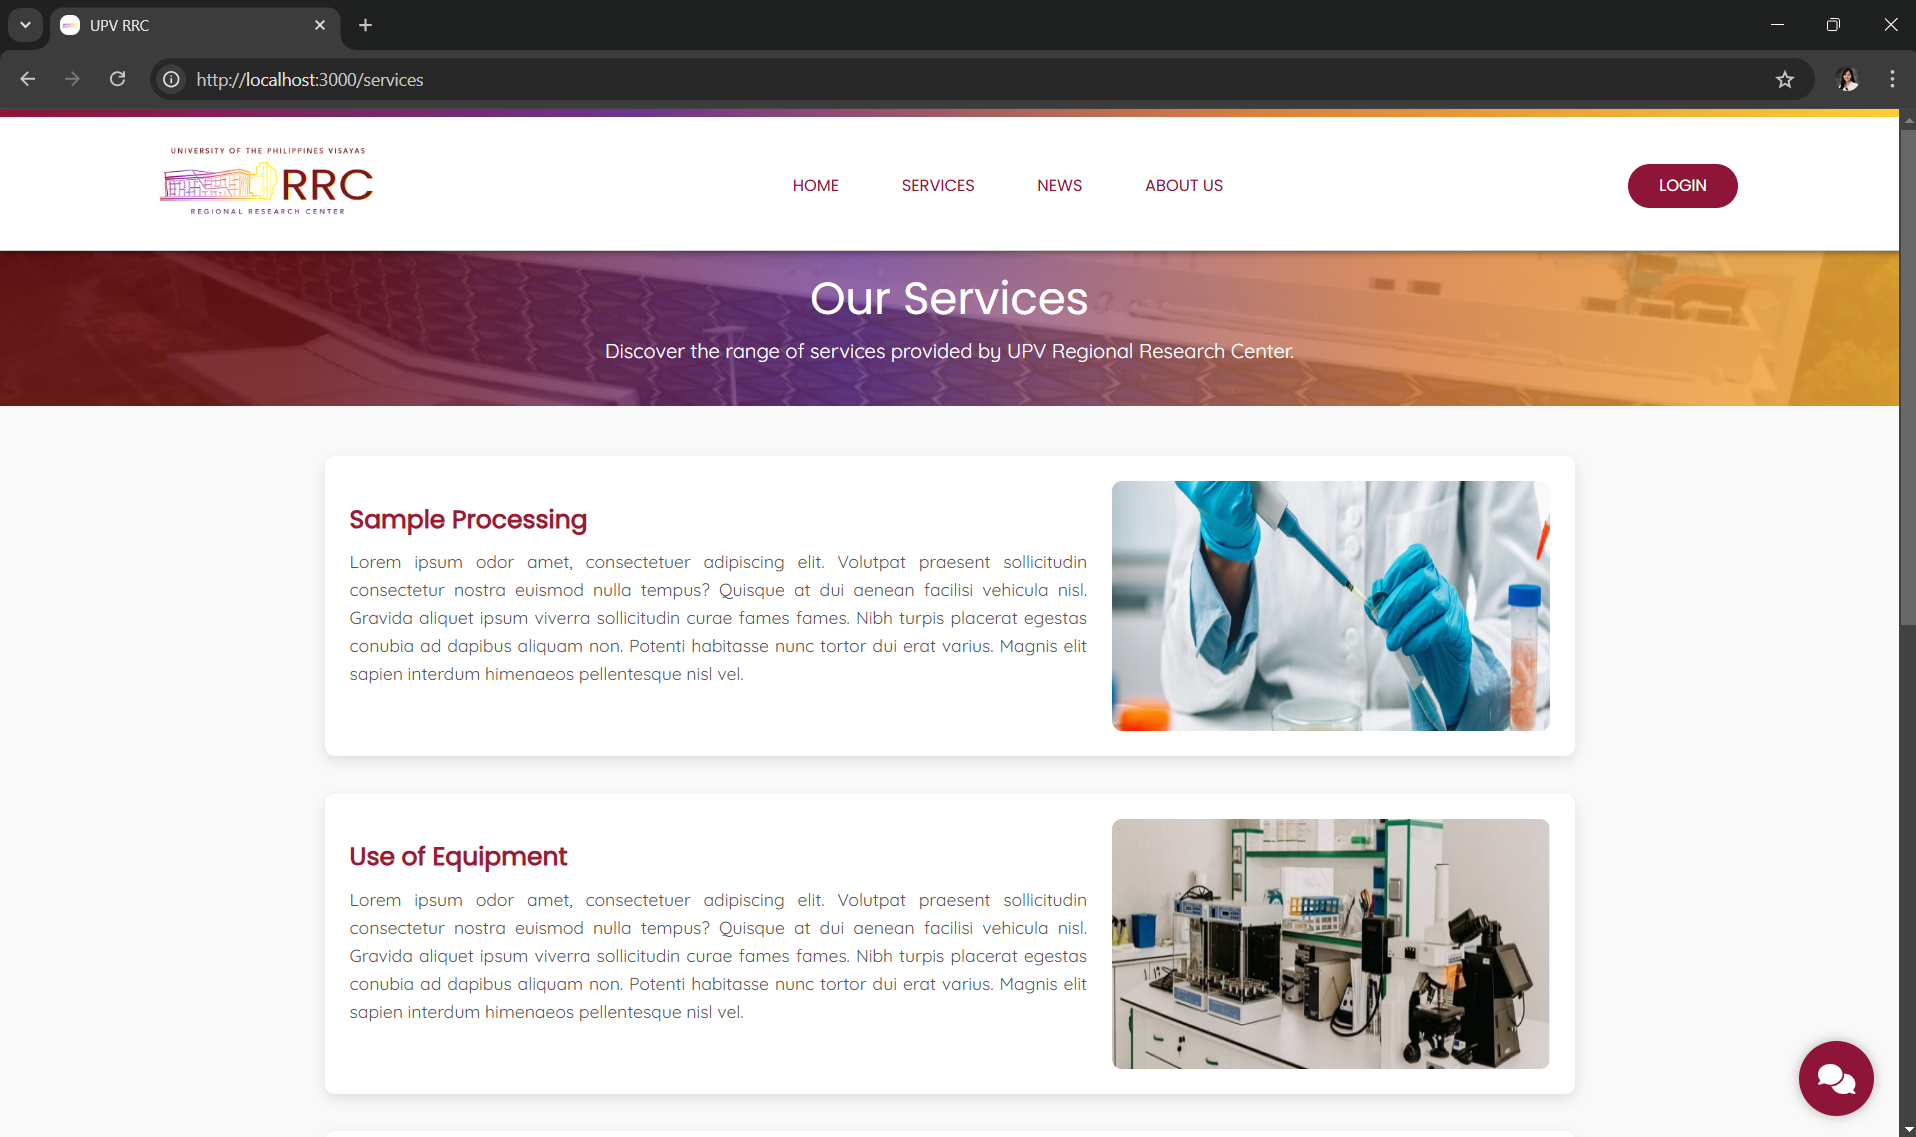
\includegraphics[width=0.75\textwidth]{service_page.png}
	\caption{Services Page}
	\label{fig:service_page}
\end{figure}

\newpage

\subsection{Laboratories Page}

Figure \ref{fig:laboratories_page} shows the `Laboratories' page. This page displays information about the laboratories within the UPV-RRC, including the available equipment and instrument for each lab. It also provides brief descriptions of each piece of equipment to give clients a better understanding of what is available. This helps the clients to make informed decisions when selecting a laboratory for their research needs. 

\begin{figure}[h]
	\centering
	
\includegraphics[width=0.8\textwidth]{laboratories.png}
	\caption{Laboratories Page}
	\label{fig:laboratories_page}
\end{figure}

\newpage

\subsection{News and Announcements Page}

Figure \ref{fig:news_page} is the `News and Announcements' page. This page serves as the central hub for all important updates related to the UPV RRC, including news about upcoming events, recent developments, announcements of new equipment or services, and relevant research highlights.The page contains two tabs, the News tab, and the Announcements tab. The News tab displays the latest news articles, while the Announcements tab contains important notices and updates from the RRC. This structure allows users to easily access and stay informed about the latest happenings at the RRC.

\begin{figure}[h]
	\centering
	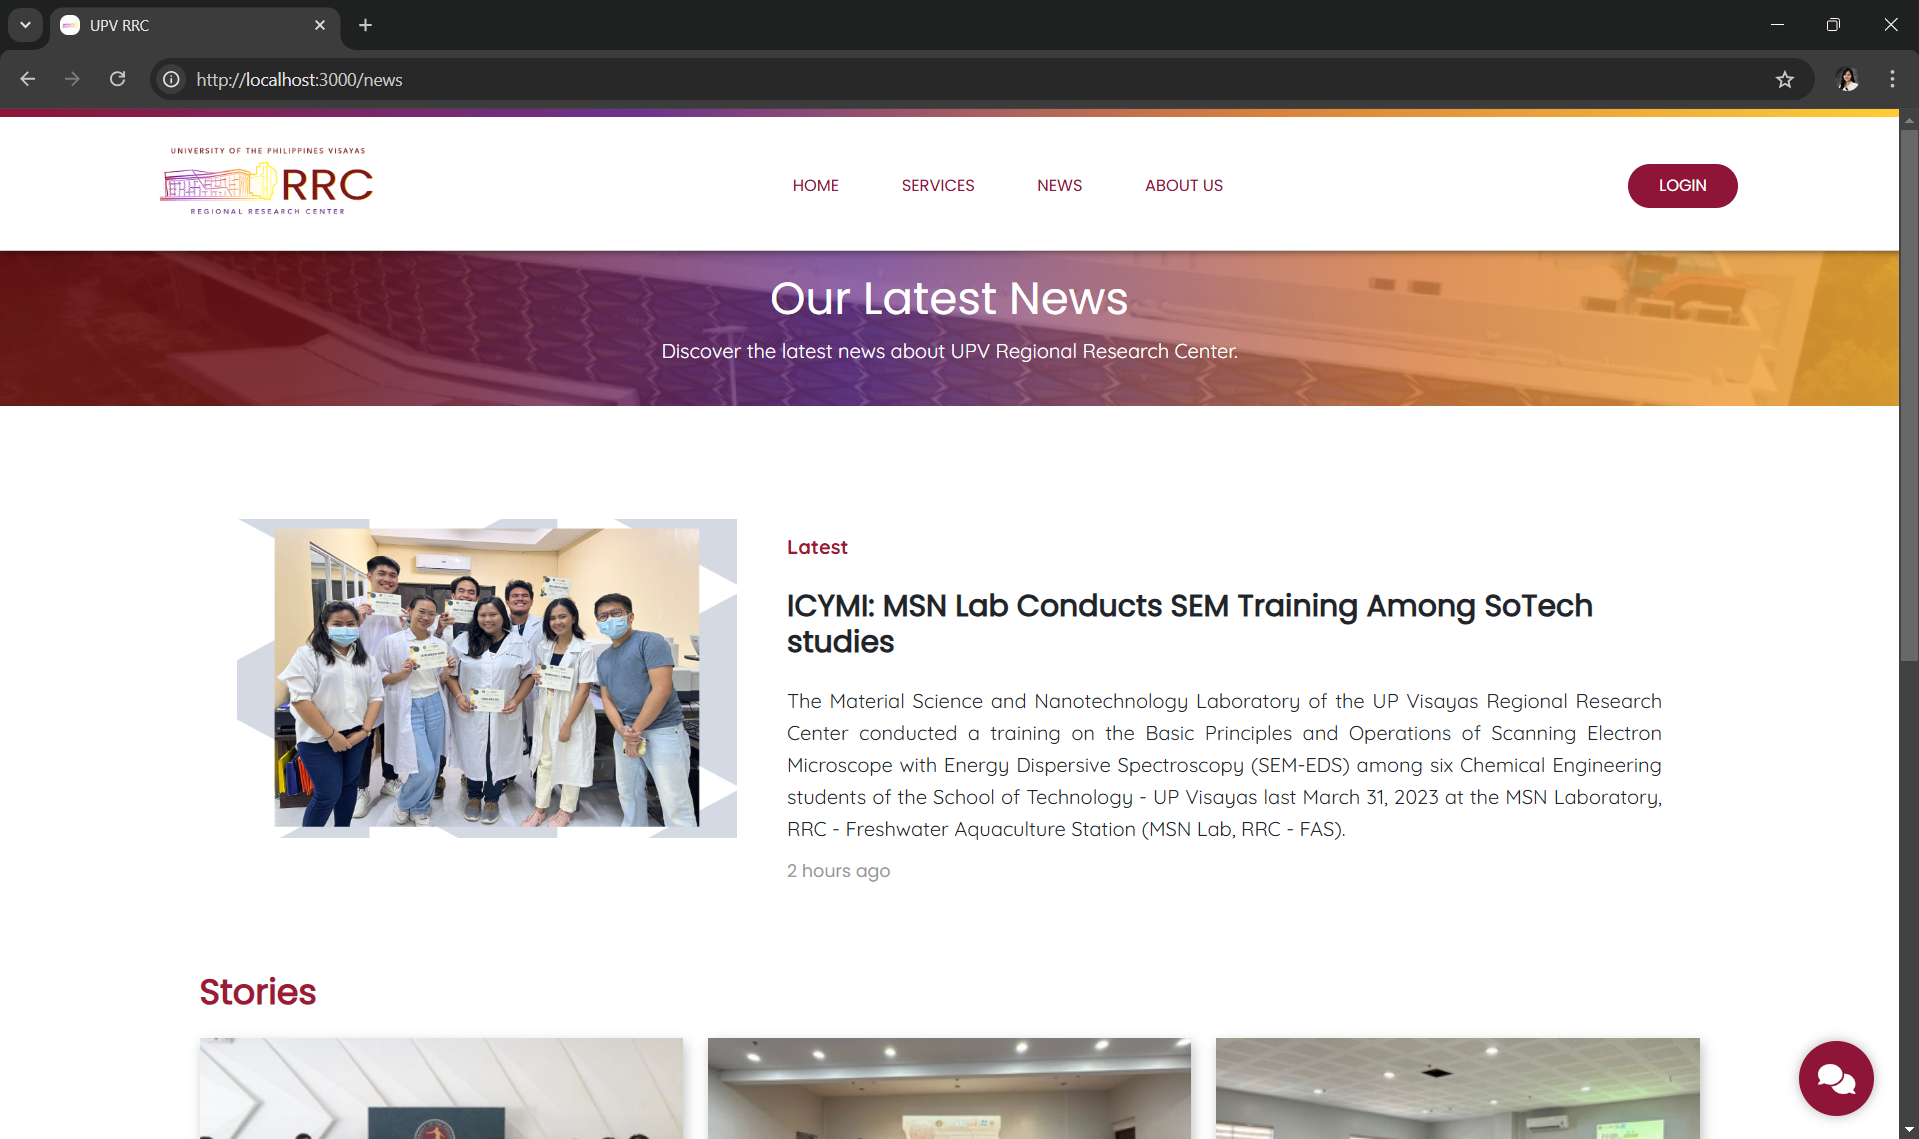
\includegraphics[width=0.7\textwidth]{news_page.png}
	\caption{News Page}
	\label{fig:news_page}
\end{figure}

\newpage

\subsection{About Us Page} 

Figure \ref{fig:about_page} shows the `About Us' page. This page provides an overview of the RRC (Regional Research Center), detailing background information, its mission, vision, and team. It is designed to give visitors a deeper understanding of the organization and its role in the research community.

\begin{figure}[h]
	\centering
	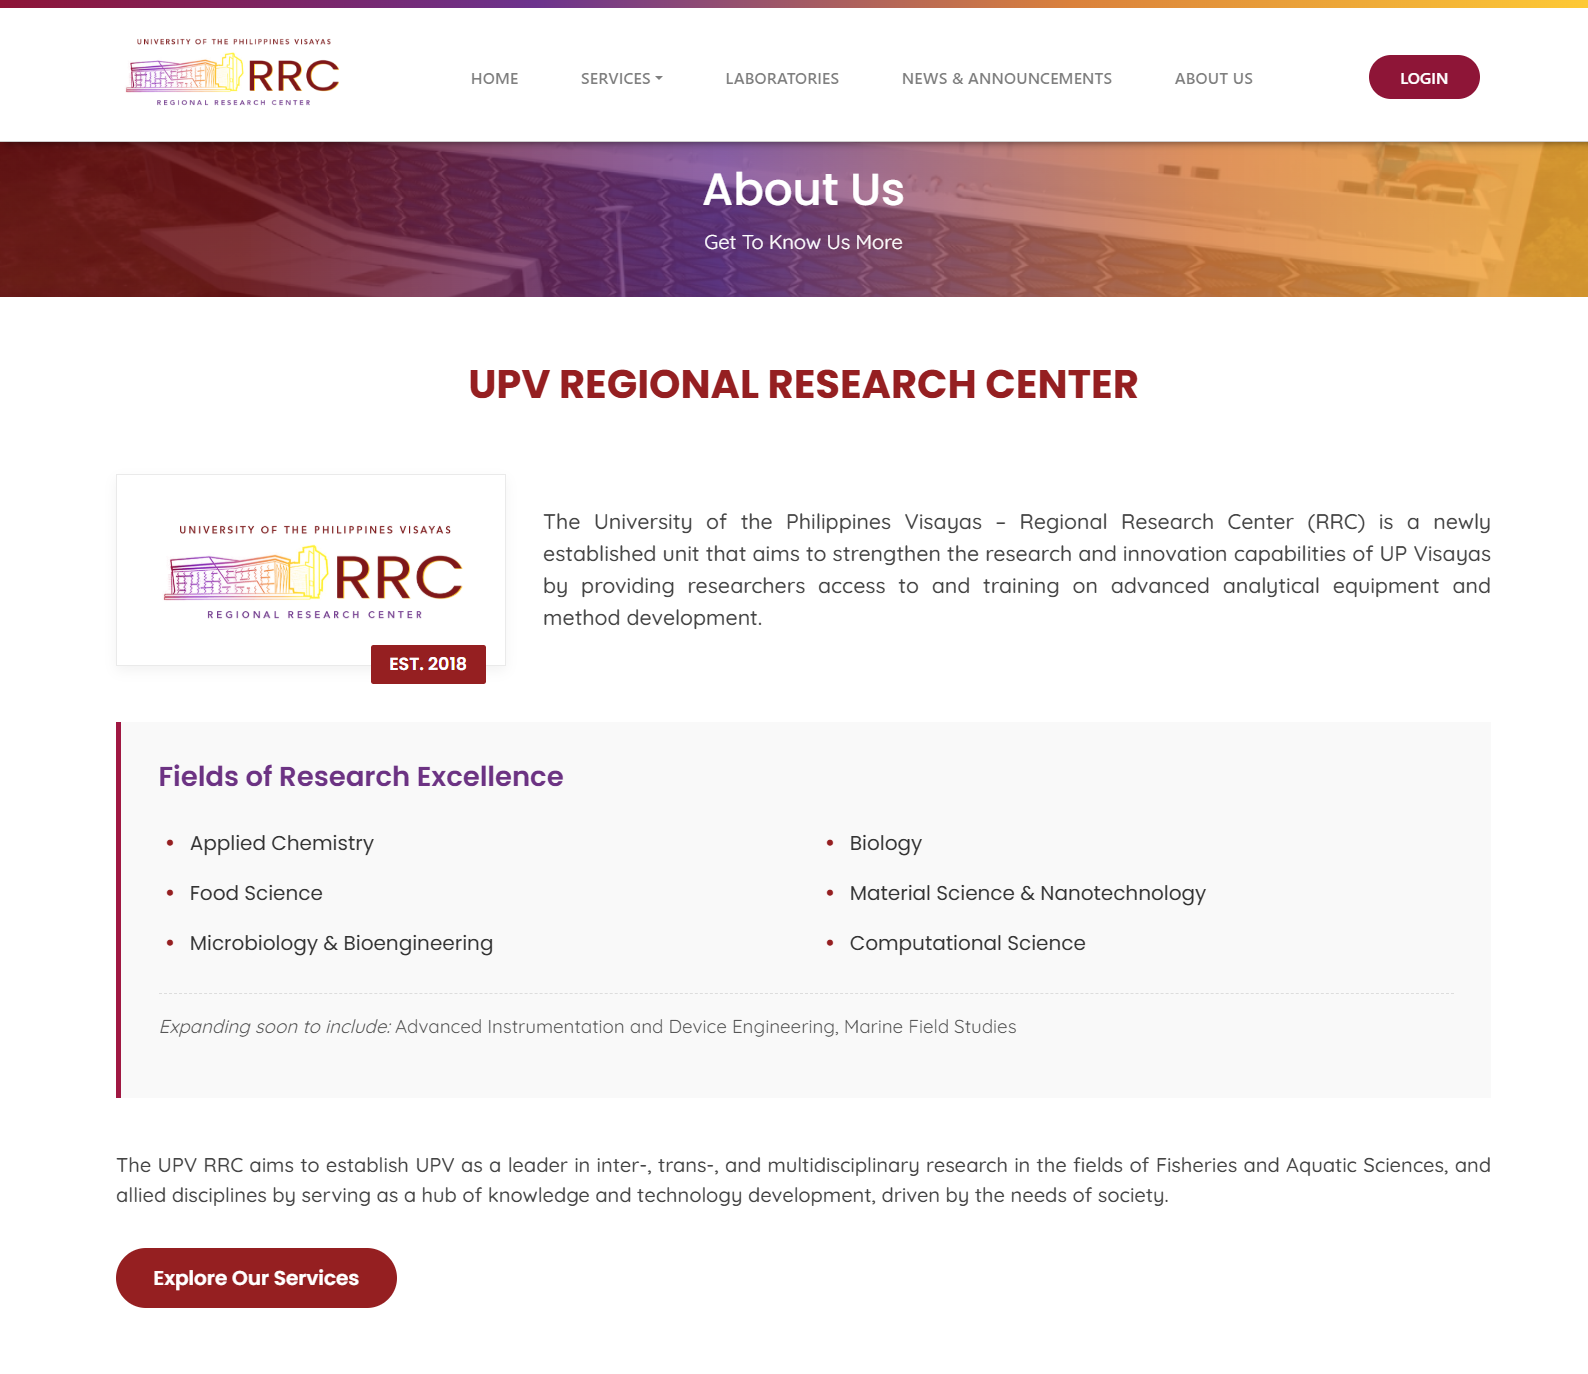
\includegraphics[width=0.8\textwidth]{about_page.png}
	\caption{About Page}
	\label{fig:about_page}
\end{figure}

\subsection{User Dashboards}

User dashboard is designed for the needs of two primary user groups of TUKIB who are the staff and clients. Each user group has a different user interface to cater to their specific needs.

\textbf{Client Dashboard}

The client dashboard is designed with simplicity and usability in mind to support individuals requesting services from the RRC. As shown in \figref{fig:client_dashboard}, the interface provides access to the client's profile, transaction history, and important reminders. A prominent “New Service Request” button is also available, allowing clients to initiate new service requests with ease. This layout ensures clients can efficiently manage their interactions with the RRC while staying informed of their request statuses.

\begin{figure}[h]
	\centering 
	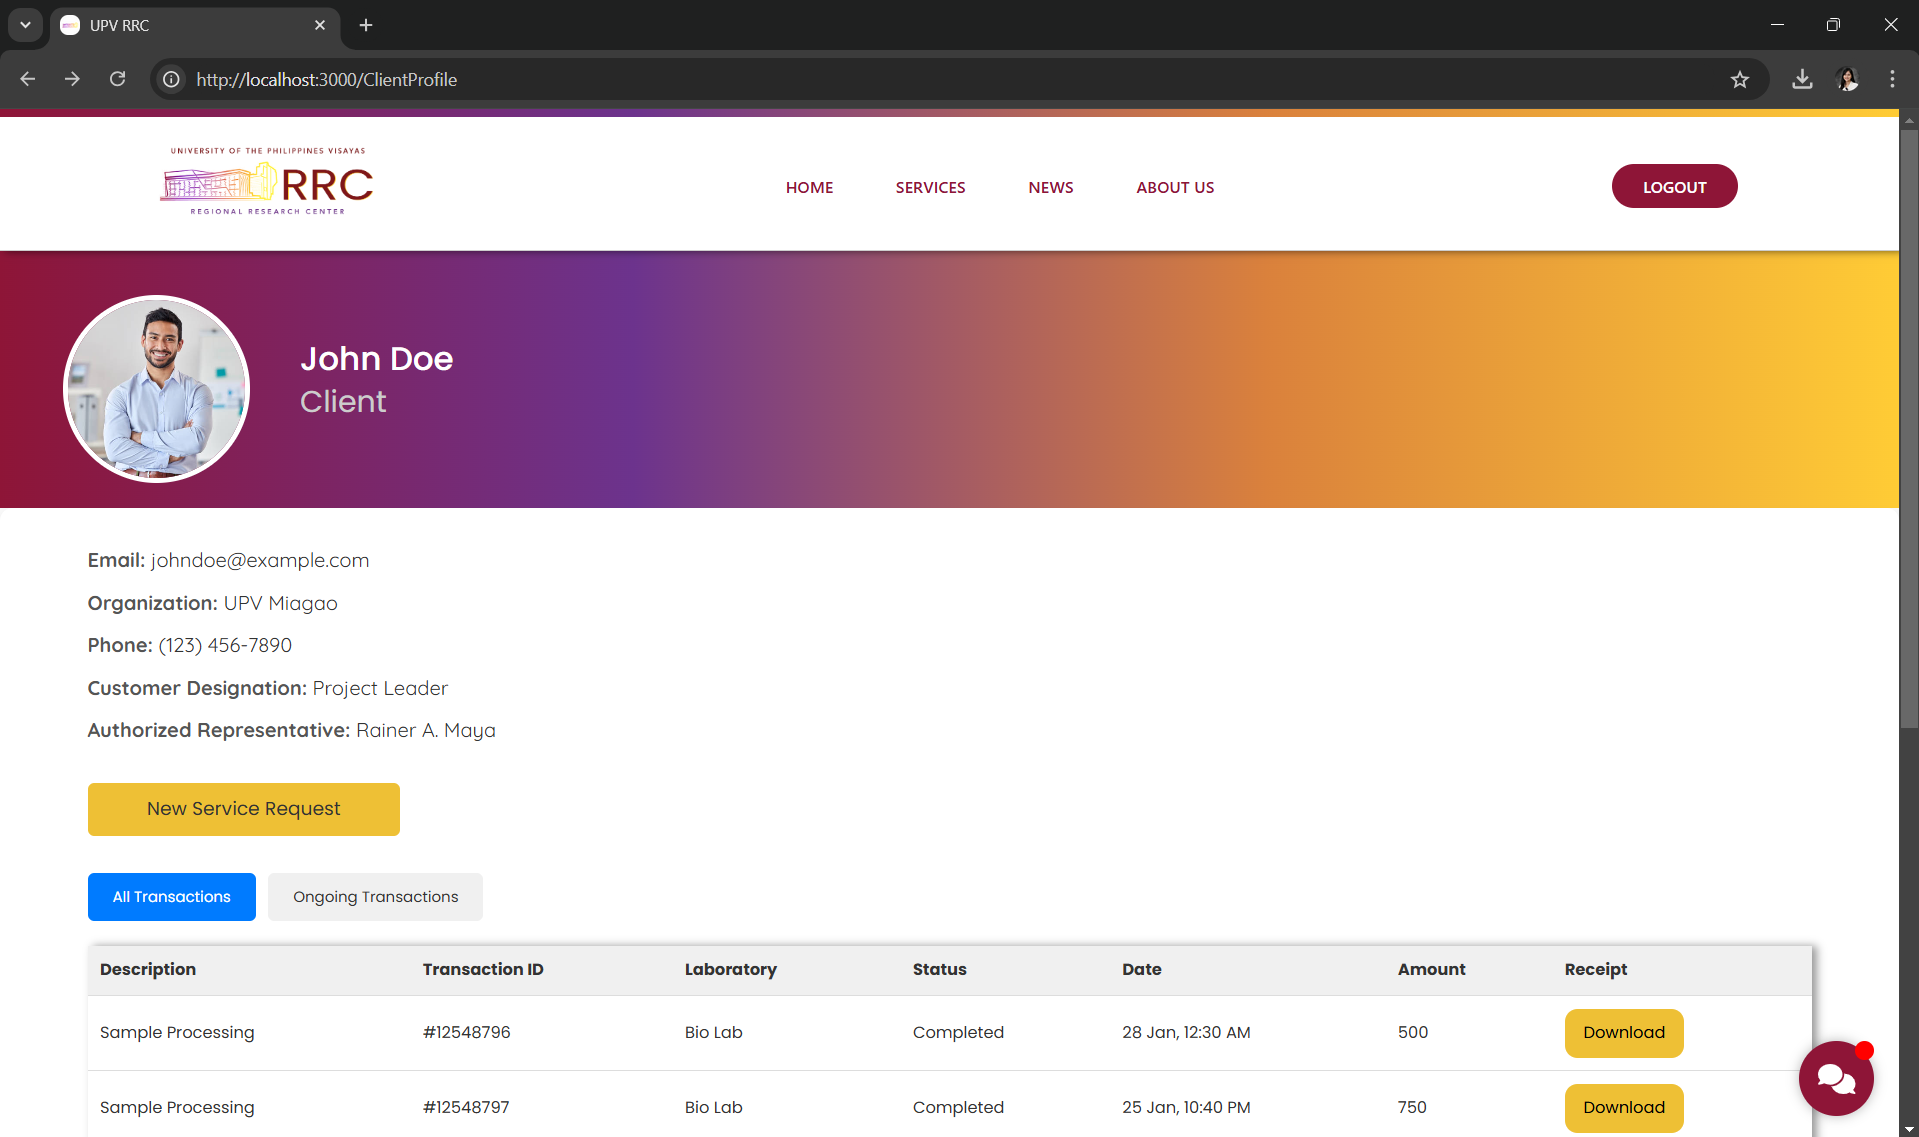
\includegraphics[width=0.8\textwidth]{client_dashboard.png}
	\caption{Client dashboard}
	\label{fig:client_dashboard}
\end{figure}

\newpage

\textbf{Staff Dashboard}

The staff dashboard is designed with role-specific functionalities, depending on the staff member's responsibilities within the RRC. \figref{fig:staff_dashboard} displays the Admin Staff dashboard, which features tabs or sections for managing different aspect of RRC's service workflow. Admin Staff can oversee all client requests, approve or reject service submissions, manage client accounts, manage laboratories, and publish news and announcements.

\begin{figure}[h]
	\centering 
	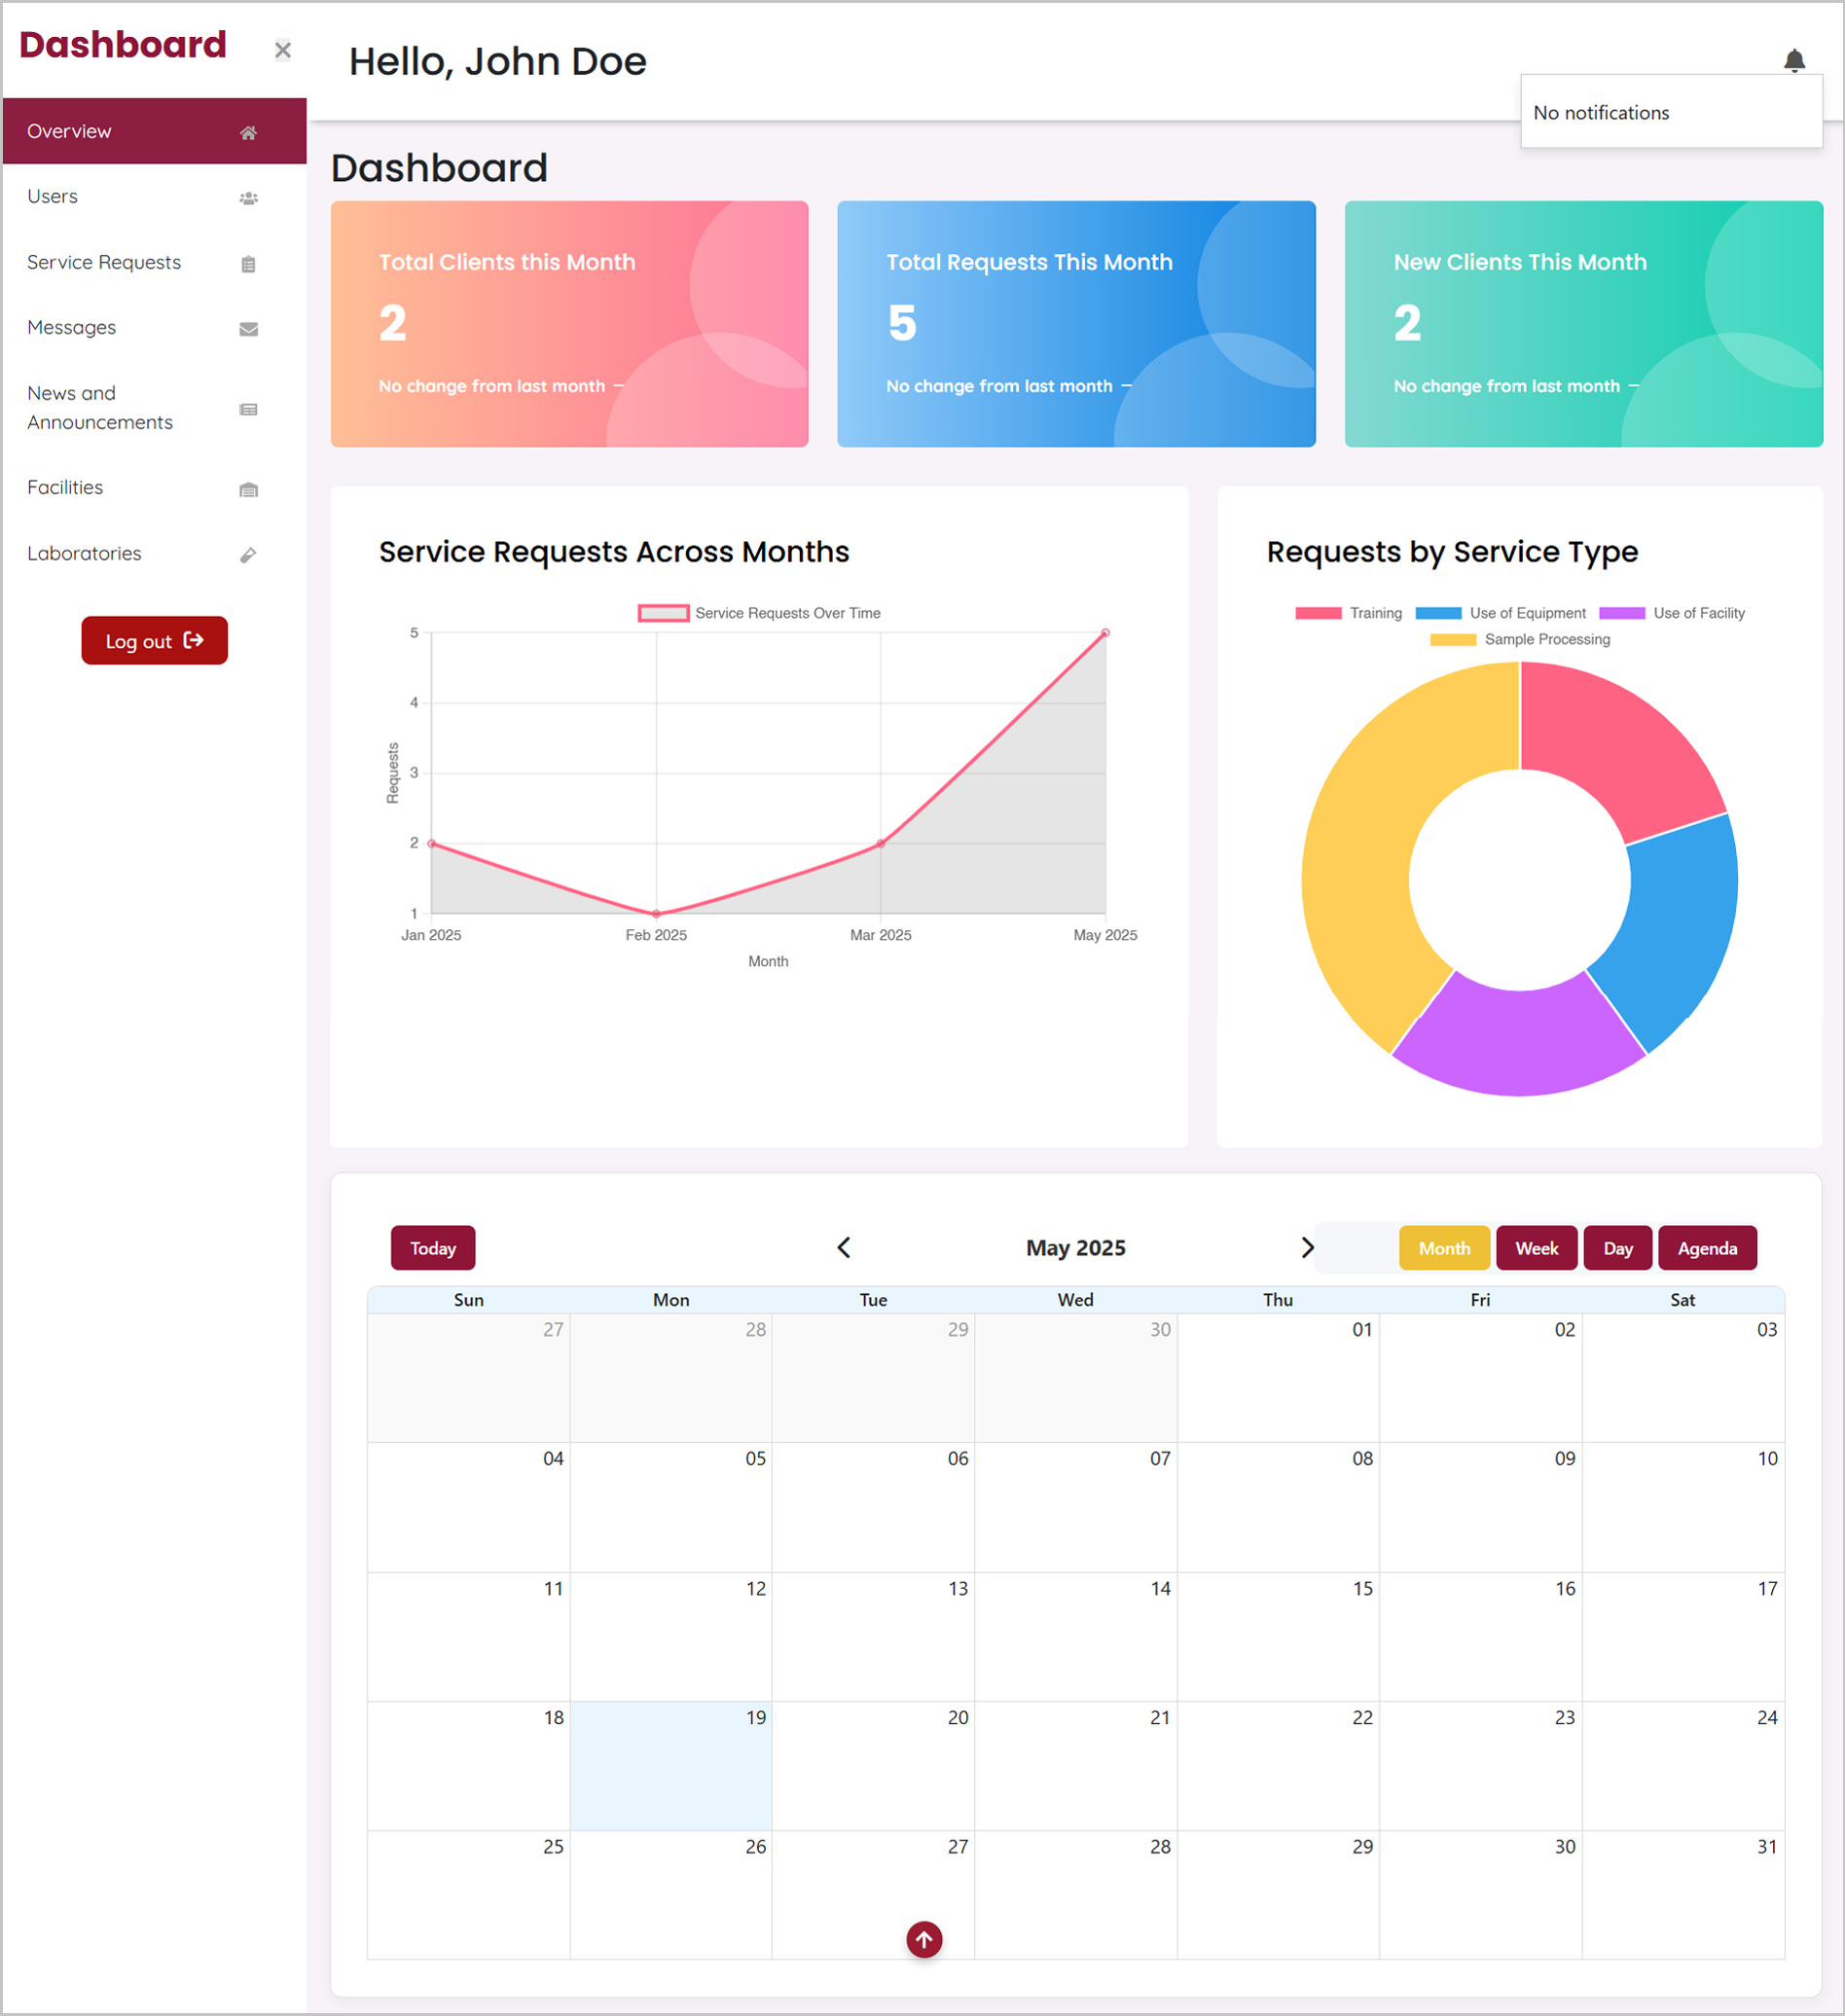
\includegraphics[width=0.8\textwidth]{staff_dashboard.png}
	\caption{Staff dashboard}
	\label{fig:staff_dashboard}
\end{figure}

For other staff members like University Researchers and TECD Staff, their dashboards present tools relevant only to their assigned workflows. This role-based design ensures each staff member can focus on their designated tasks without distractions from unrelated features, improving efficiency and clarity.

\section{System Features}

\subsection{User Management Module}

\textbf{User registration}

Clients can create their own accounts through the sign in page. However, by default, these accounts will remain inactive until the Admin Staff approves them after reviewing their information. An additional step is required in which they must undergo an initial consultation with the staff. Only after this consultation will their account be permitted to submit a service request. This process ensures that new clients are informed about the proper procedures for requesting a service, as consultation is a necessary step.

To reinforce this requirement, as shown on figure \figref{fig:signup_popup}, a pop-up reminder is shown when the sign-up page loads, displaying the message: 
\textit{"Note: Before signing up, please make sure you have completed the initial consultation with RRC. This step is required to proceed with account creation."}
Users, are required to acknowledge this reminder by clicking the "Ok, I Understand" button before they proceed with the sign-up process.
Additionally, a reminder is displayed beside the sign up form stating: 
\textit{"ACCOUNT REGISTRATION IS ONLY AVAILABLE AFTER AN INITIAL CONSULTATION. PLEASE CONSULT WITH RRC FIRST VIA EMAIL TO PROCEED."} 
These ensure that users are aware of the necessary steps before creating an account, thus preventing premature registrations without prior consultation.

\begin{figure}[h]
	\centering 
	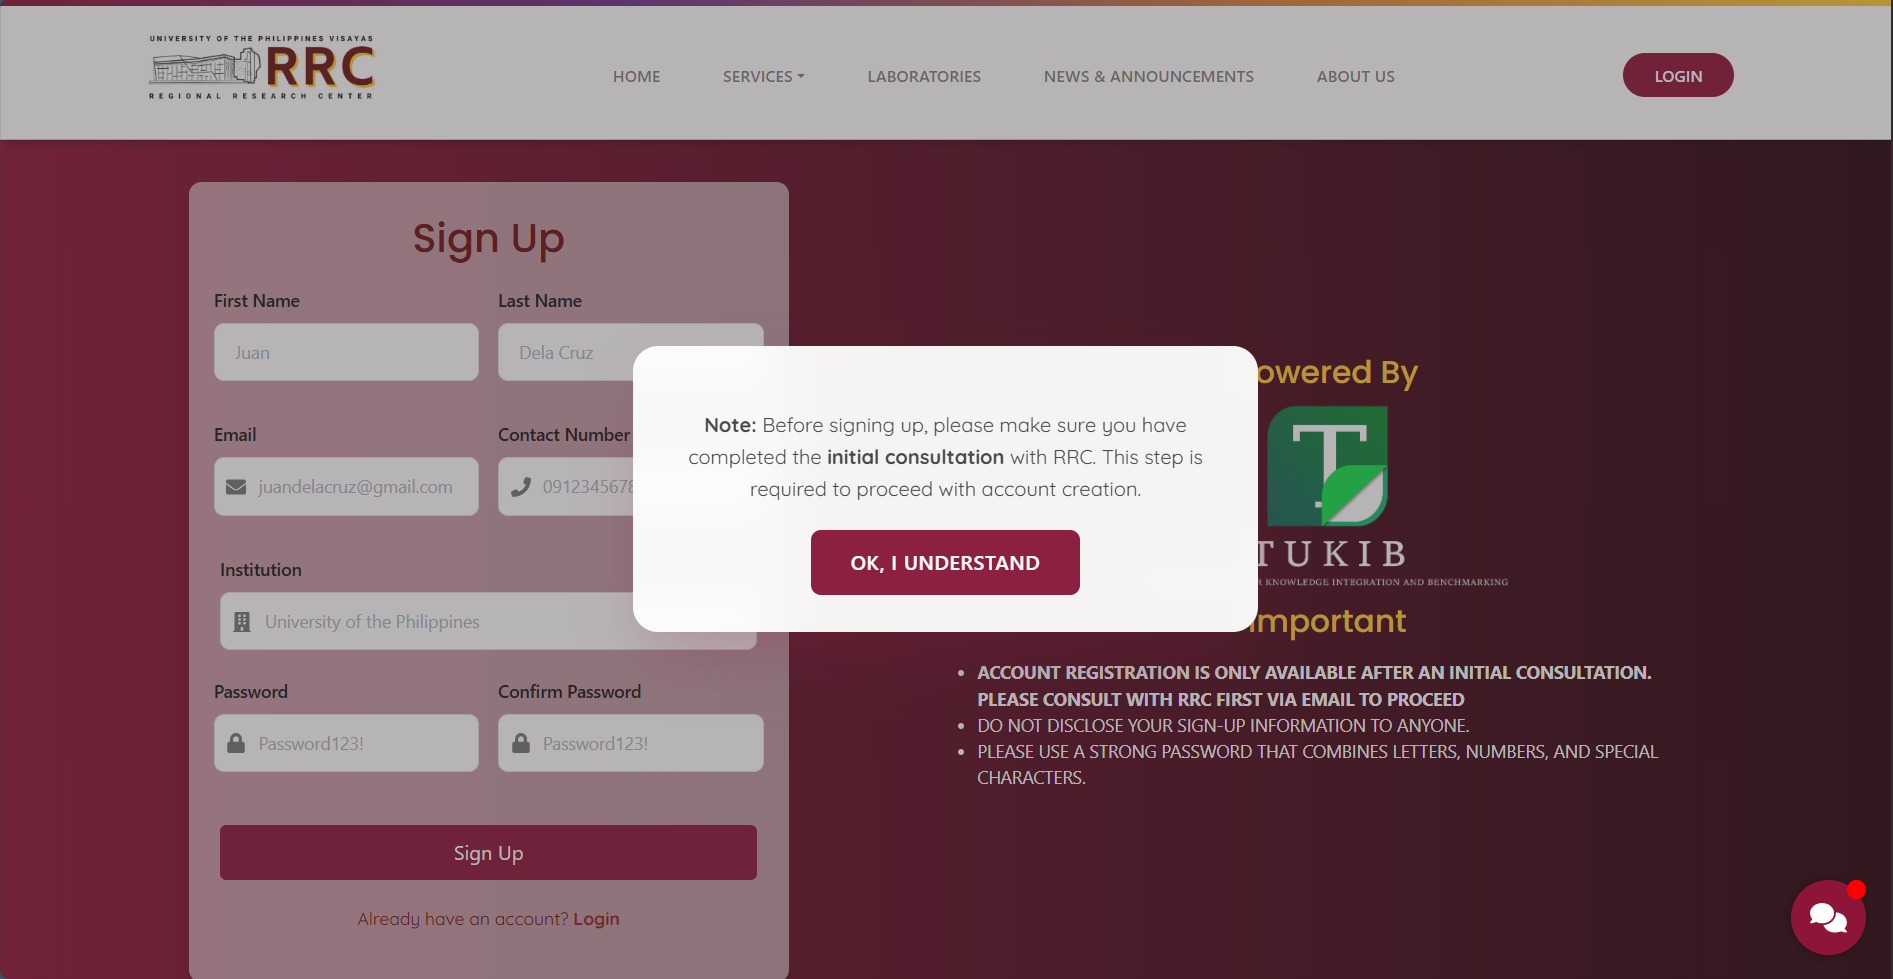
\includegraphics[width=0.8\textwidth]{signup_popup.png}
	\caption{Sign-Up Pop-Up Reminder}
	\label{fig:signup_popup}
\end{figure}

As shown in \figref{fig:signup_page}, the sign-up page collects essential information such as the client's full name, email (used to notify them when their account is approved and becomes active), contact number, institution, and a password. This ensures that the system gathers all relevant details needed for account verification and further communication. Proper input validation mechanisms are also in place to ensure data integrity—for example, email addresses must be unique to prevent duplicate accounts, and all required fields must be properly filled before submission.

On the other hand, staff accounts are pre-made by the Admin Staff. This approach ensures that only authorized personnel are granted access to the system’s internal functions, promoting security and controlled user management.

\newpage

\begin{figure}[h]
	\centering 
	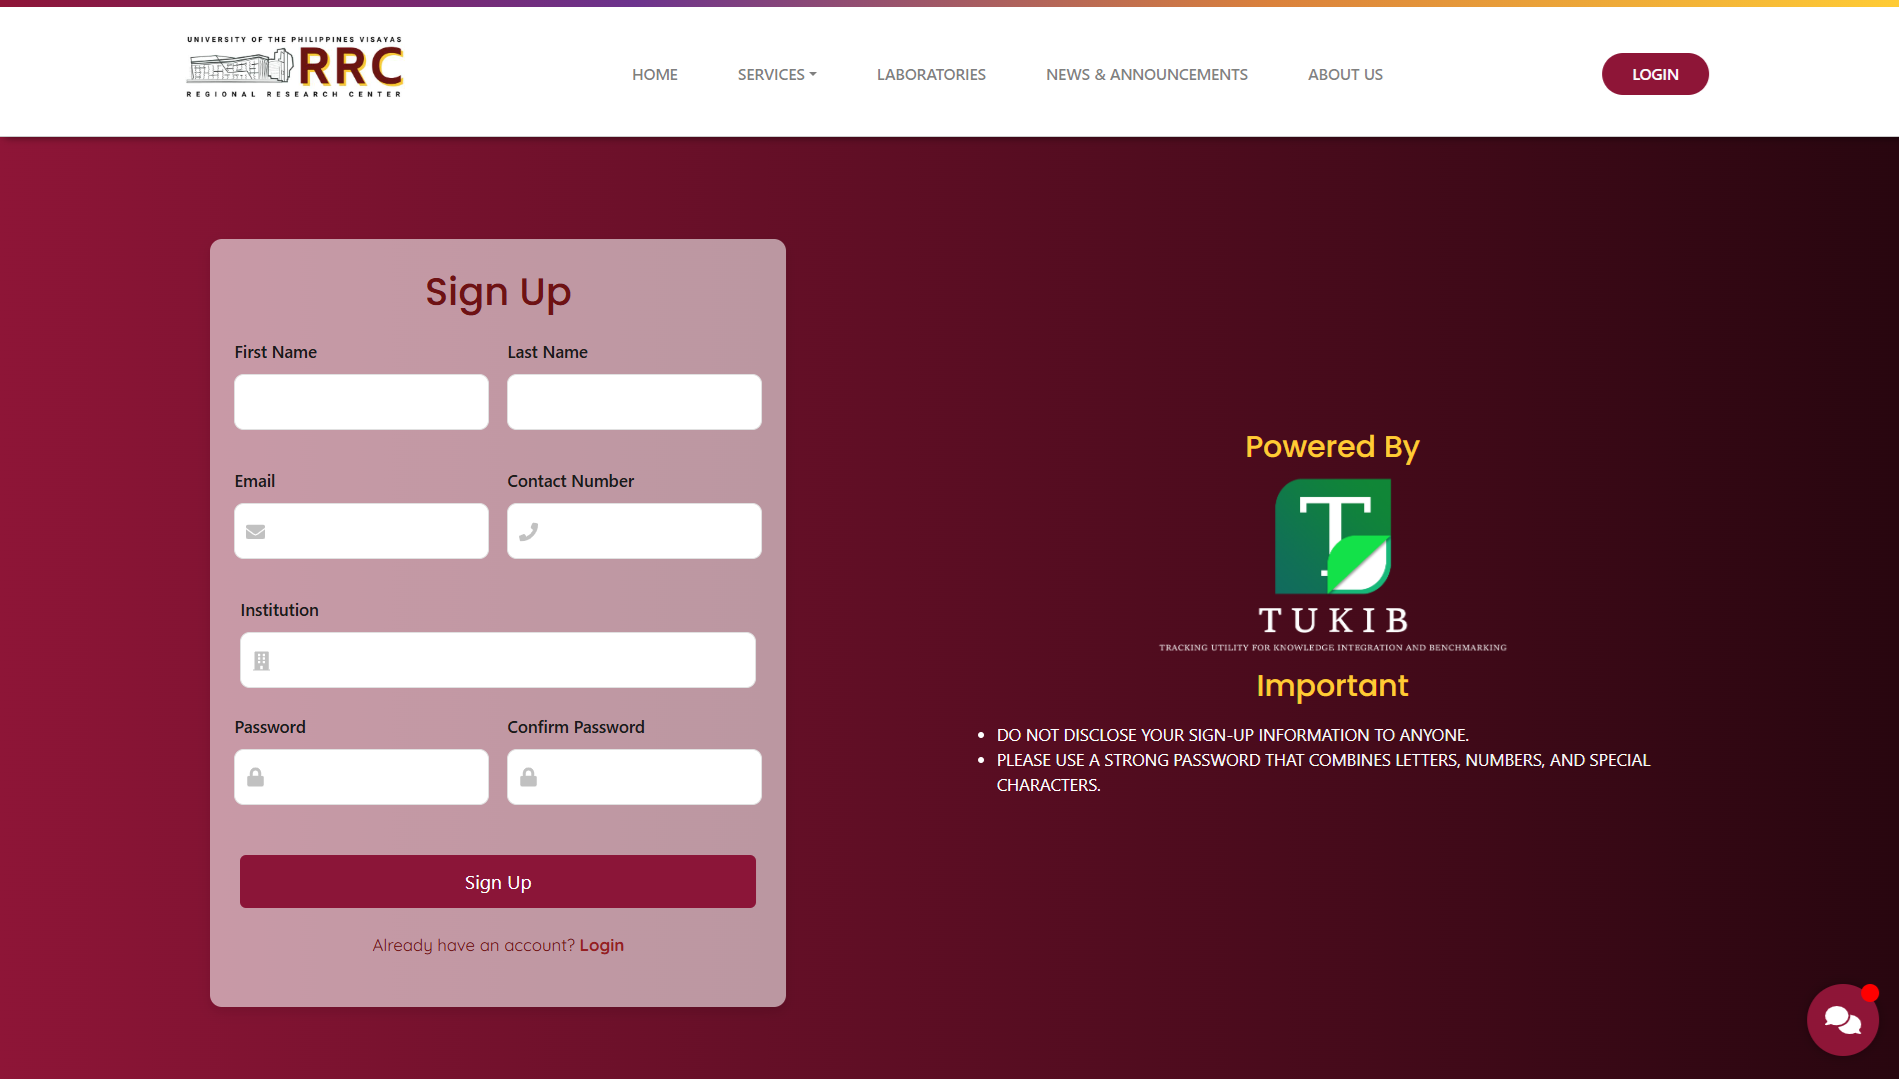
\includegraphics[width=0.8\textwidth]{sign_up.png}
	\caption{Sign Up Page}
	\label{fig:signup_page}
\end{figure}

\textbf{User authentication}

On the login page, users need to enter their email address and password. Additionally, Google authentication is available, allowing users to sign in using their Google account for a quicker and more secure login experience. Passwords are hidden by default, but users can click the eye icon in the password field (as shown in \figref{fig:login}) to toggle visibility. After successfully logging in, users will be redirected to their respective dashboards.

\begin{figure}[h]
	\centering 
	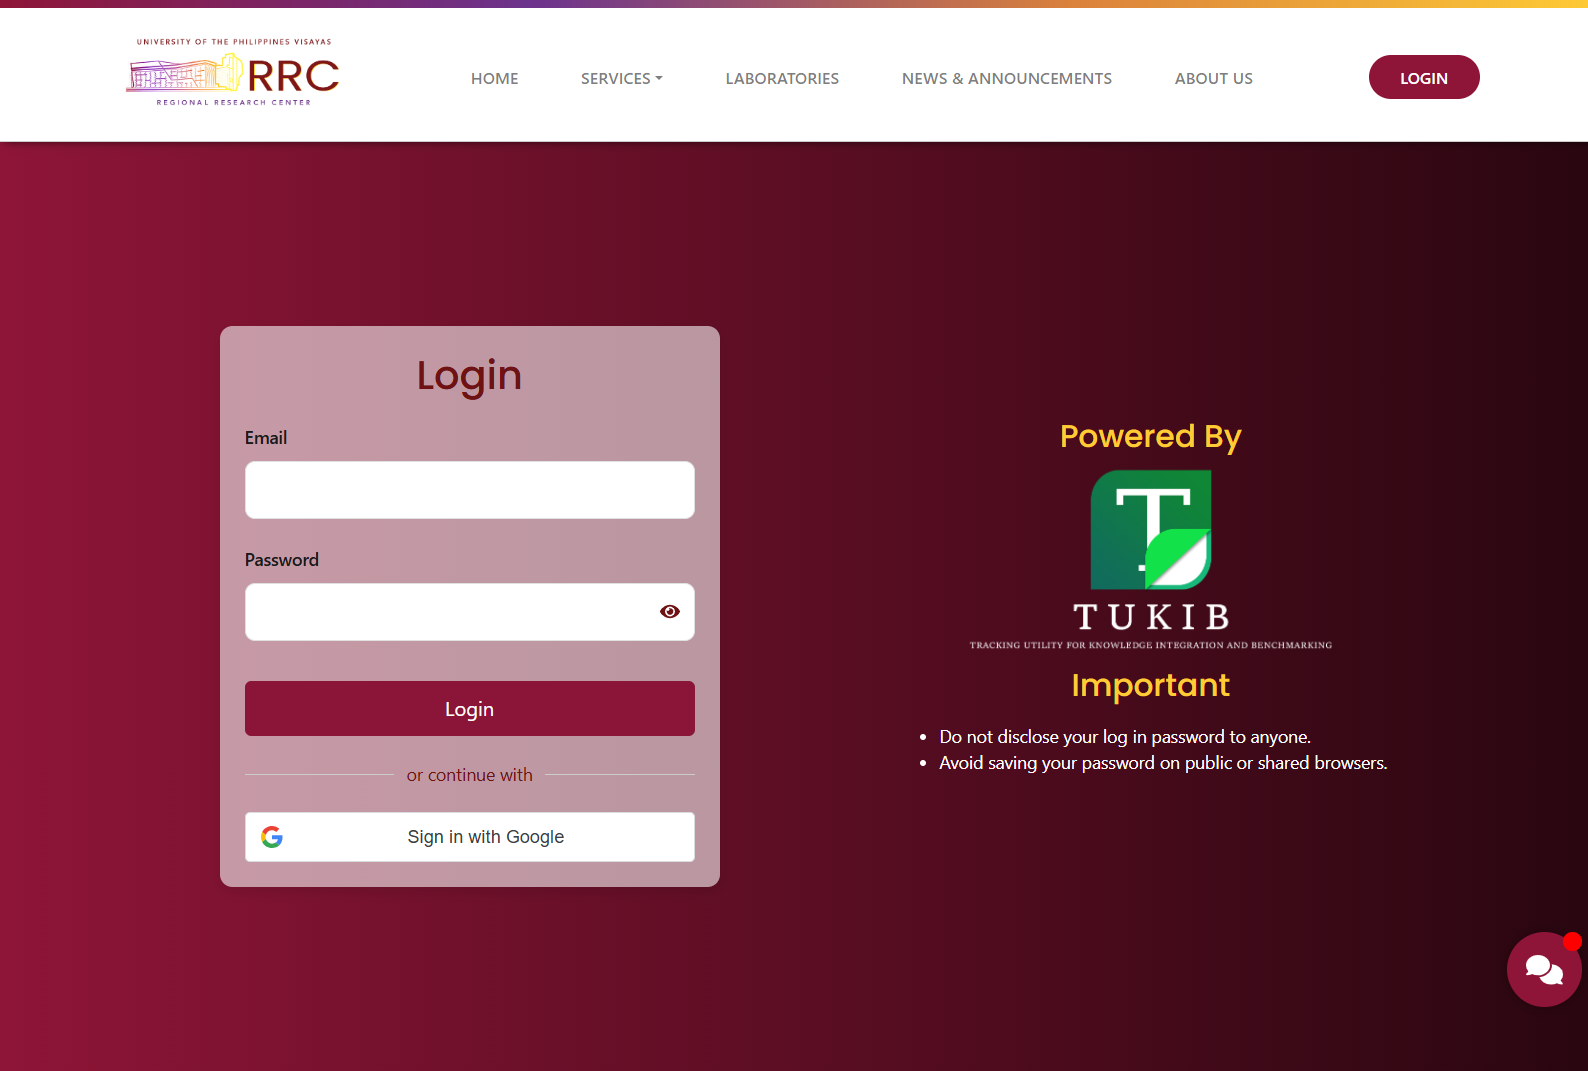
\includegraphics[width=0.8\textwidth]{login.png}
	\caption{Log In Page}
	\label{fig:login}
\end{figure}

\subsection{Service Request Module}

One of the core features of TUKIB is the Service Request Module, which enables both clients and staff to efficiently access, track, and manage service requests through their respective accounts. Clients can submit service requests, monitor the status of their requests, upload payment receipts, view results, and provide feedback to the UPV Regional Research Center. On the other hand, staff members have the capability to approve or reject requests, update request statuses, upload charge slips and results, and review payment receipts submitted by clients. This bidirectional functionality ensures that each request is processed smoothly from initiation to completion.

The service request form, shown in \figref{fig:form_tooltips_placeholders}, is designed to be user-friendly and intuitive. It includes fields for entering the type of service requested, a description of the request, and all other necessary information required by the RRC. The form also features tooltips and placeholder texts to guide users in filling out the necessary information correctly. This helps reduce errors and ensures that all required details are provided before submission.

\begin{figure}[h]
	\centering 
	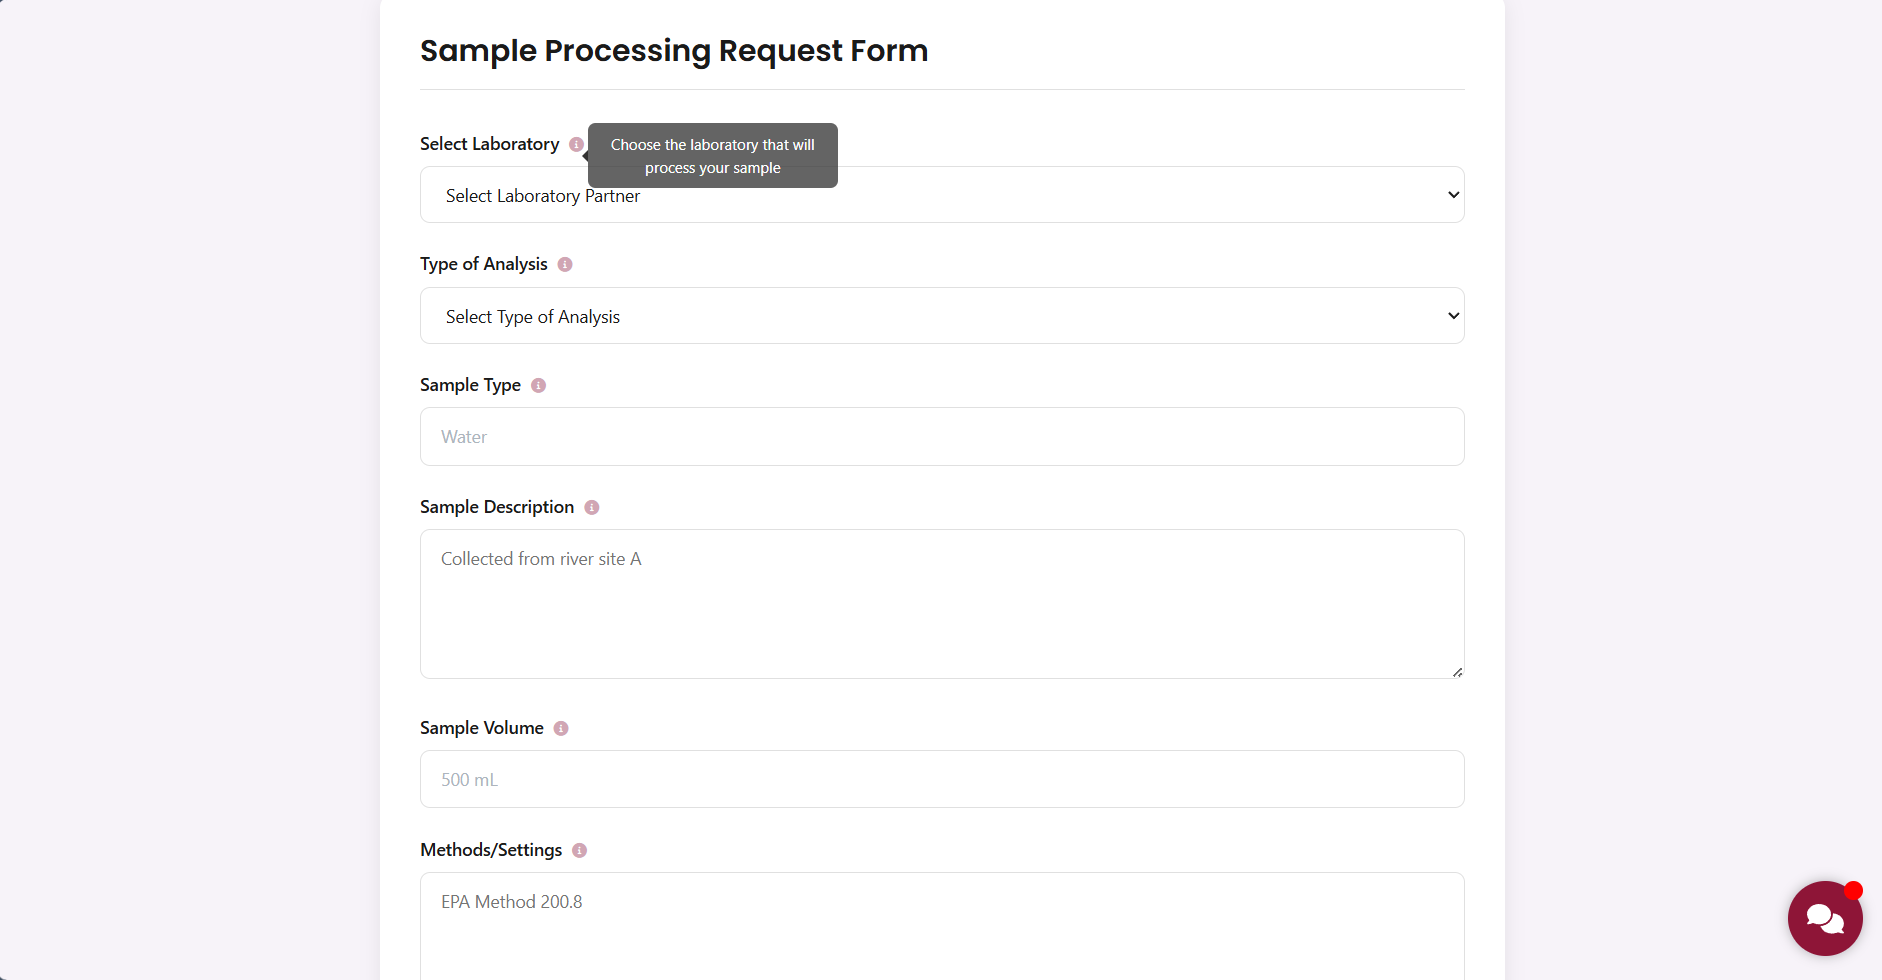
\includegraphics[width=0.75\textwidth]{form_tooltips_placeholders.png}
	\caption{Service Request Form Showing Tooltips and Placeholder Texts}
	\label{fig:form_tooltips_placeholders}
\end{figure}

\newpage

\figref{fig:service_request_details} displays the full service request details page. This page contains comprehensive information about a specific request and is accessible to both clients and staff, depending on their role. It includes key details such as the type of service requested, current status, payment information, and required documents. A progress indicator is also provided to help both parties track the current stage of the request.

Additionally, role-based functionalities are implemented to tailor the interface to each user's responsibilities. For instance, staff users can approve requests, generate charge slips, and upload final results. Meanwhile, clients can upload payment receipts, view results, and provide feedback.

\newpage

\begin{figure}[h]
	\centering 
	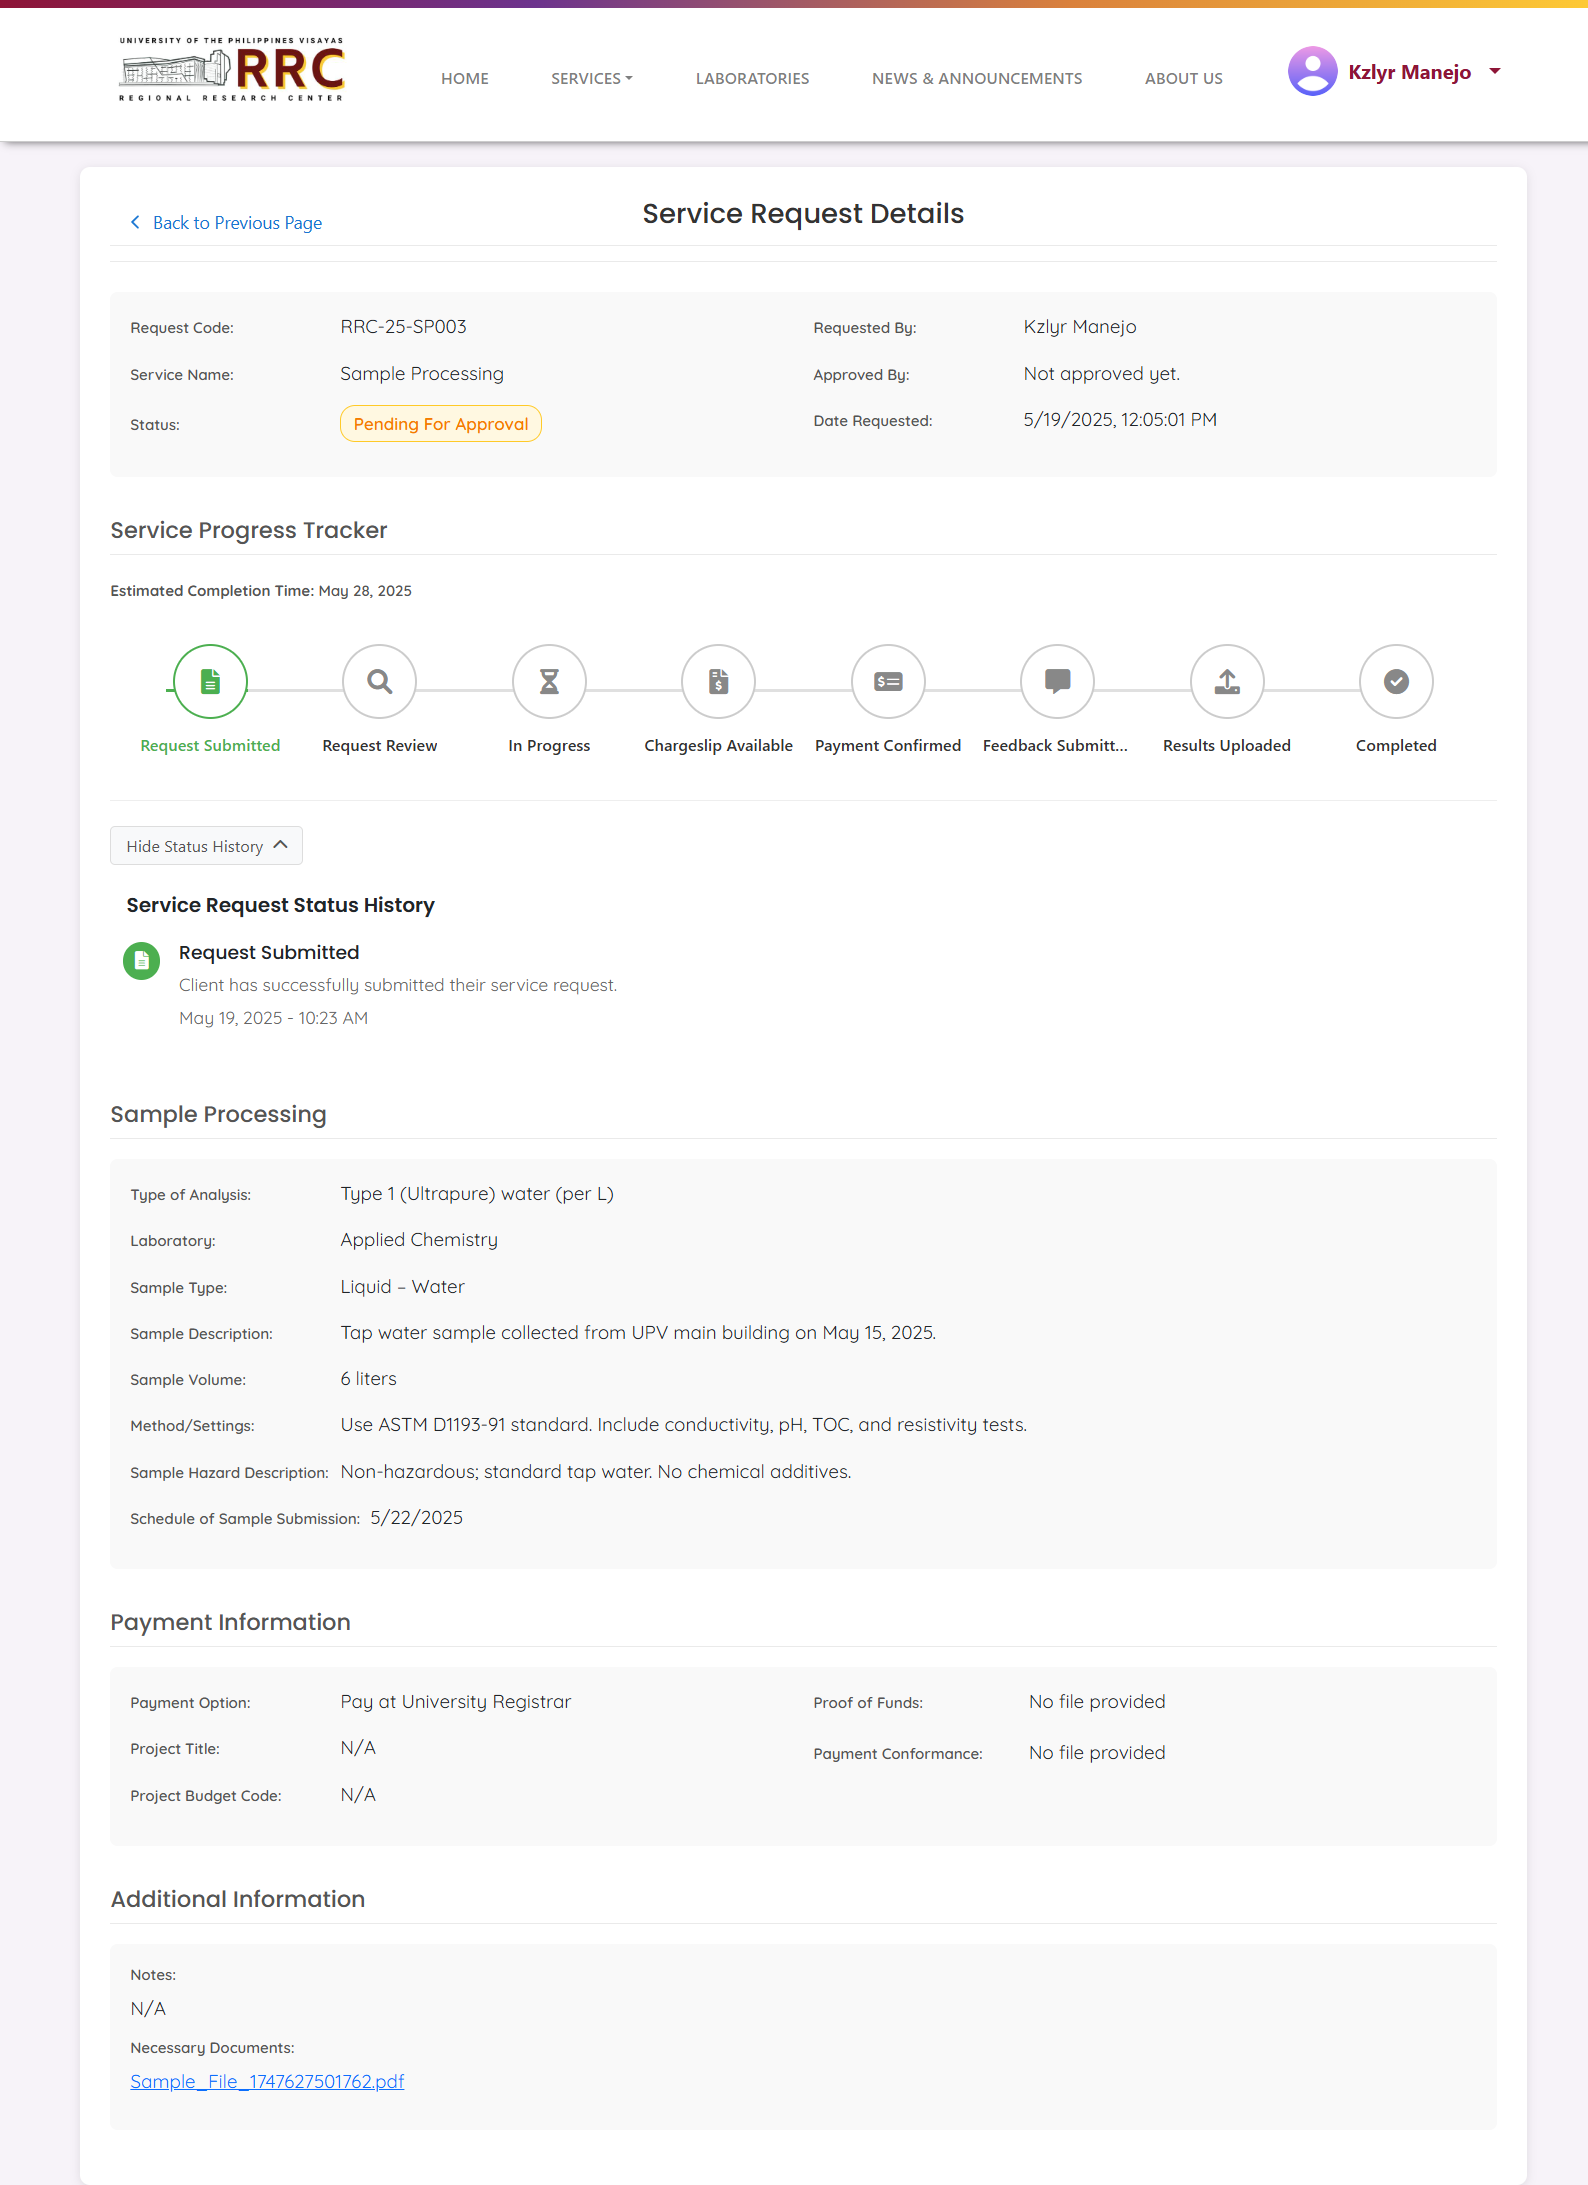
\includegraphics[width=0.75\textwidth]{service_request_details.png}
	\caption{Service Request Details Page}
	\label{fig:service_request_details}
\end{figure}

\newpage

\subsection{Calendar and Scheduling Module}

To effectively manage service schedules, TUKIB includes a Calendar and Scheduling Module. This enables staff to view and track scheduled services in a clear and organized format. There are four types of calendars within the system: general, laboratory, equipment, and facility.

The general calendar serves as an overview of all the institution's activities. When a date is marked as unavailable or restricted in the system calendar— may it be due to holidays, maintenance, or other events—it is automatically blocked across all laboratory, equipment, and facility calendars, preventing any requests from client for that date. This calendar is managed by the Admin Staff and Director.

The calendar for laboratory is designed for managing schedules specific to each laboratory. Every laboratory has its own dedicated calendar displaying unavailable dates and available date and time slots. University Researchers overseeing a laboratory can optionally choose to include some or all equipment, within the laboratory, under the same scheduling restrictions when managing service availability.

In addition, each piece of equipment has its own calendar to track availability. This helps prevent double bookings. Similarly, each Facility, such as conference rooms or audio/visual rooms, has its own calendar to manage usage and avoid scheduling conflicts.

All calendars are interactive and updated in real time. Changes such as request approvals, rejections, or cancellations are reflected immediately, allowing users and staff to make informed decisions and avoid scheduling conflicts.

The calendar is interactive and updated in real time, ensuring that any unavailability or availability is communicated across staff and clients. This module enhances transparency, supports better planning, and contributes to a smoother service flow within TUKIB.

Figure~\ref{fig:calendar} shows the calendar interface within the system. When a date is clicked, a form will be shown asking for necessary details regarding its unavailability of the date.

\begin{figure}[h]
    \centering
    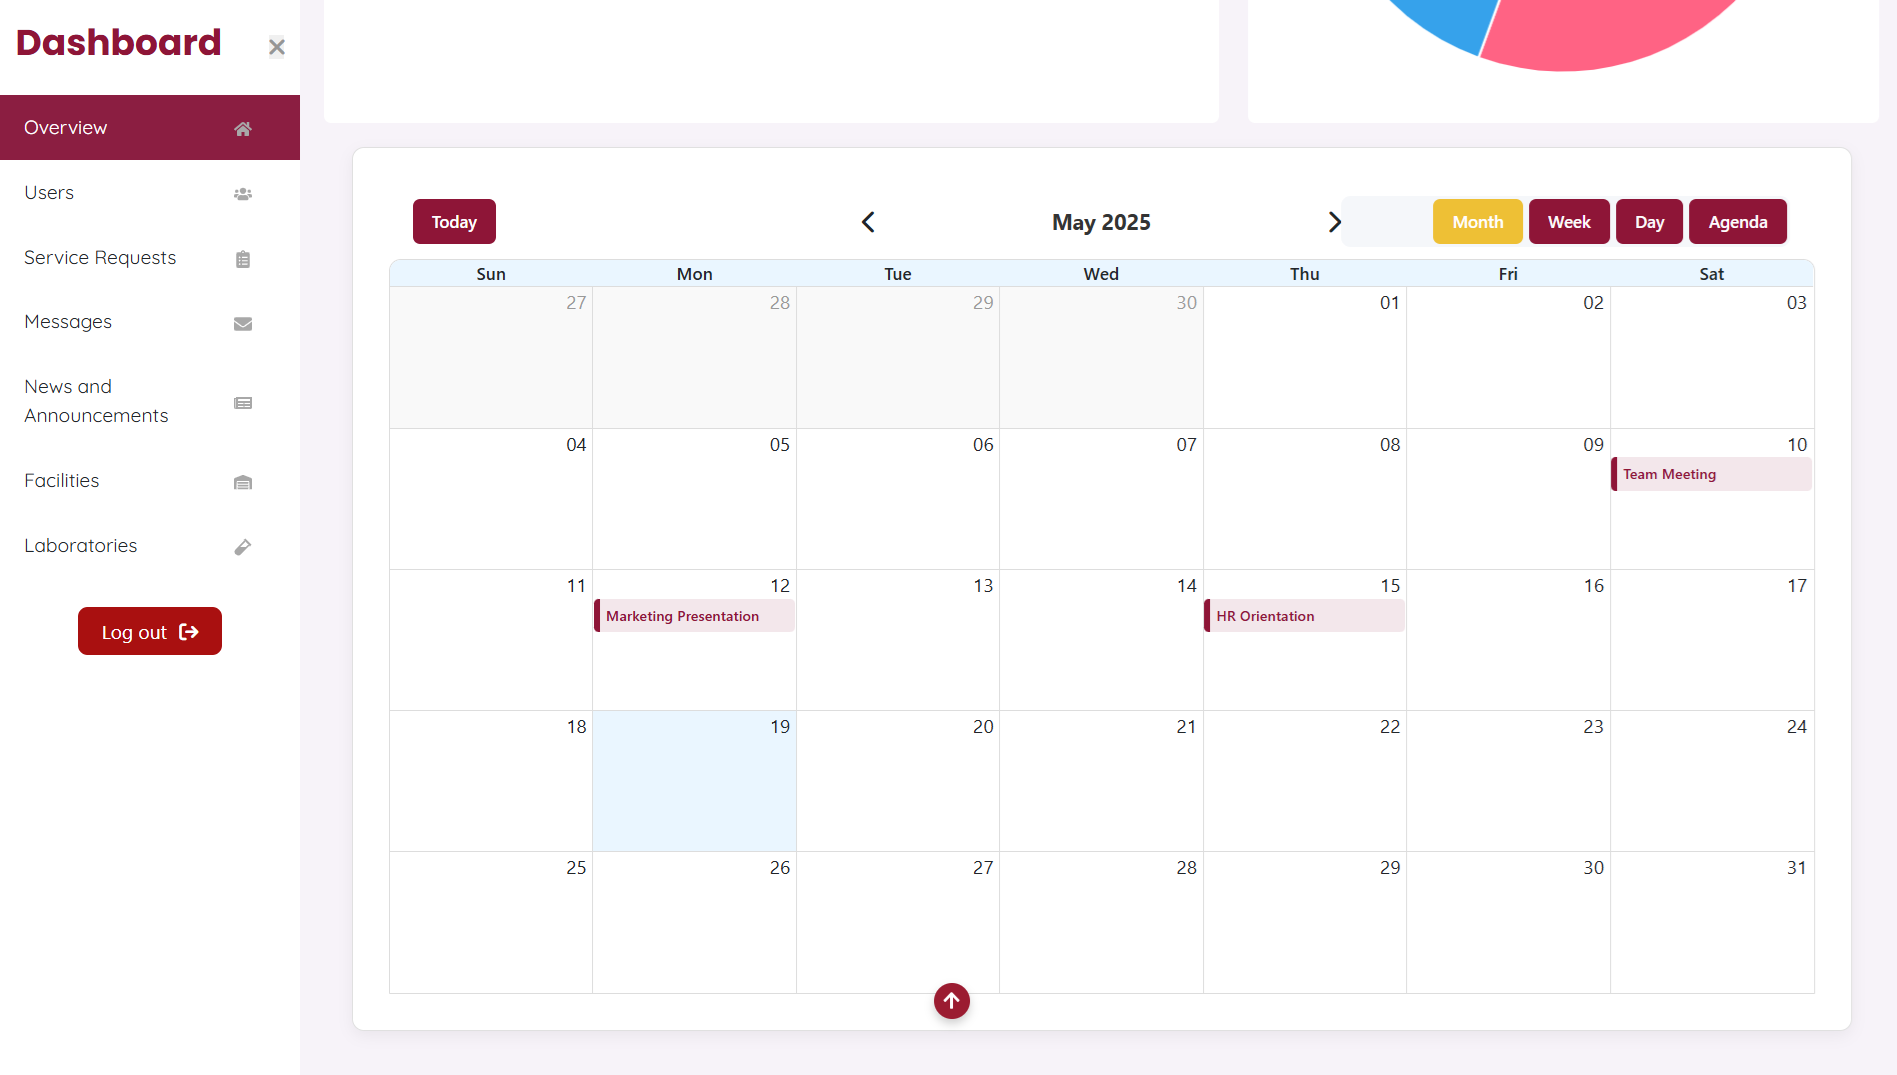
\includegraphics[width=0.8\textwidth]{calendar.png}
    \caption{Calendar}
    \label{fig:calendar}
\end{figure}

\newpage

\subsection{News and Announcement Module}

To facilitate efficient communication between the RRC and its stakeholders, the system features a News and Announcement Module. This allows Admin Staff and TECD Staff to create and post important public updates, news, and announcements directly within the platform, particularly those related to the RRC and its services.

As seen in \figref{fig:announcements}, the module provides fields for entering a title, composing the content, and uploading relevant images. This ensures that relevant information such as upcoming RRC events, service changes, and newly available equipment is effectively communicated.

\begin{figure}[h]
    \centering
    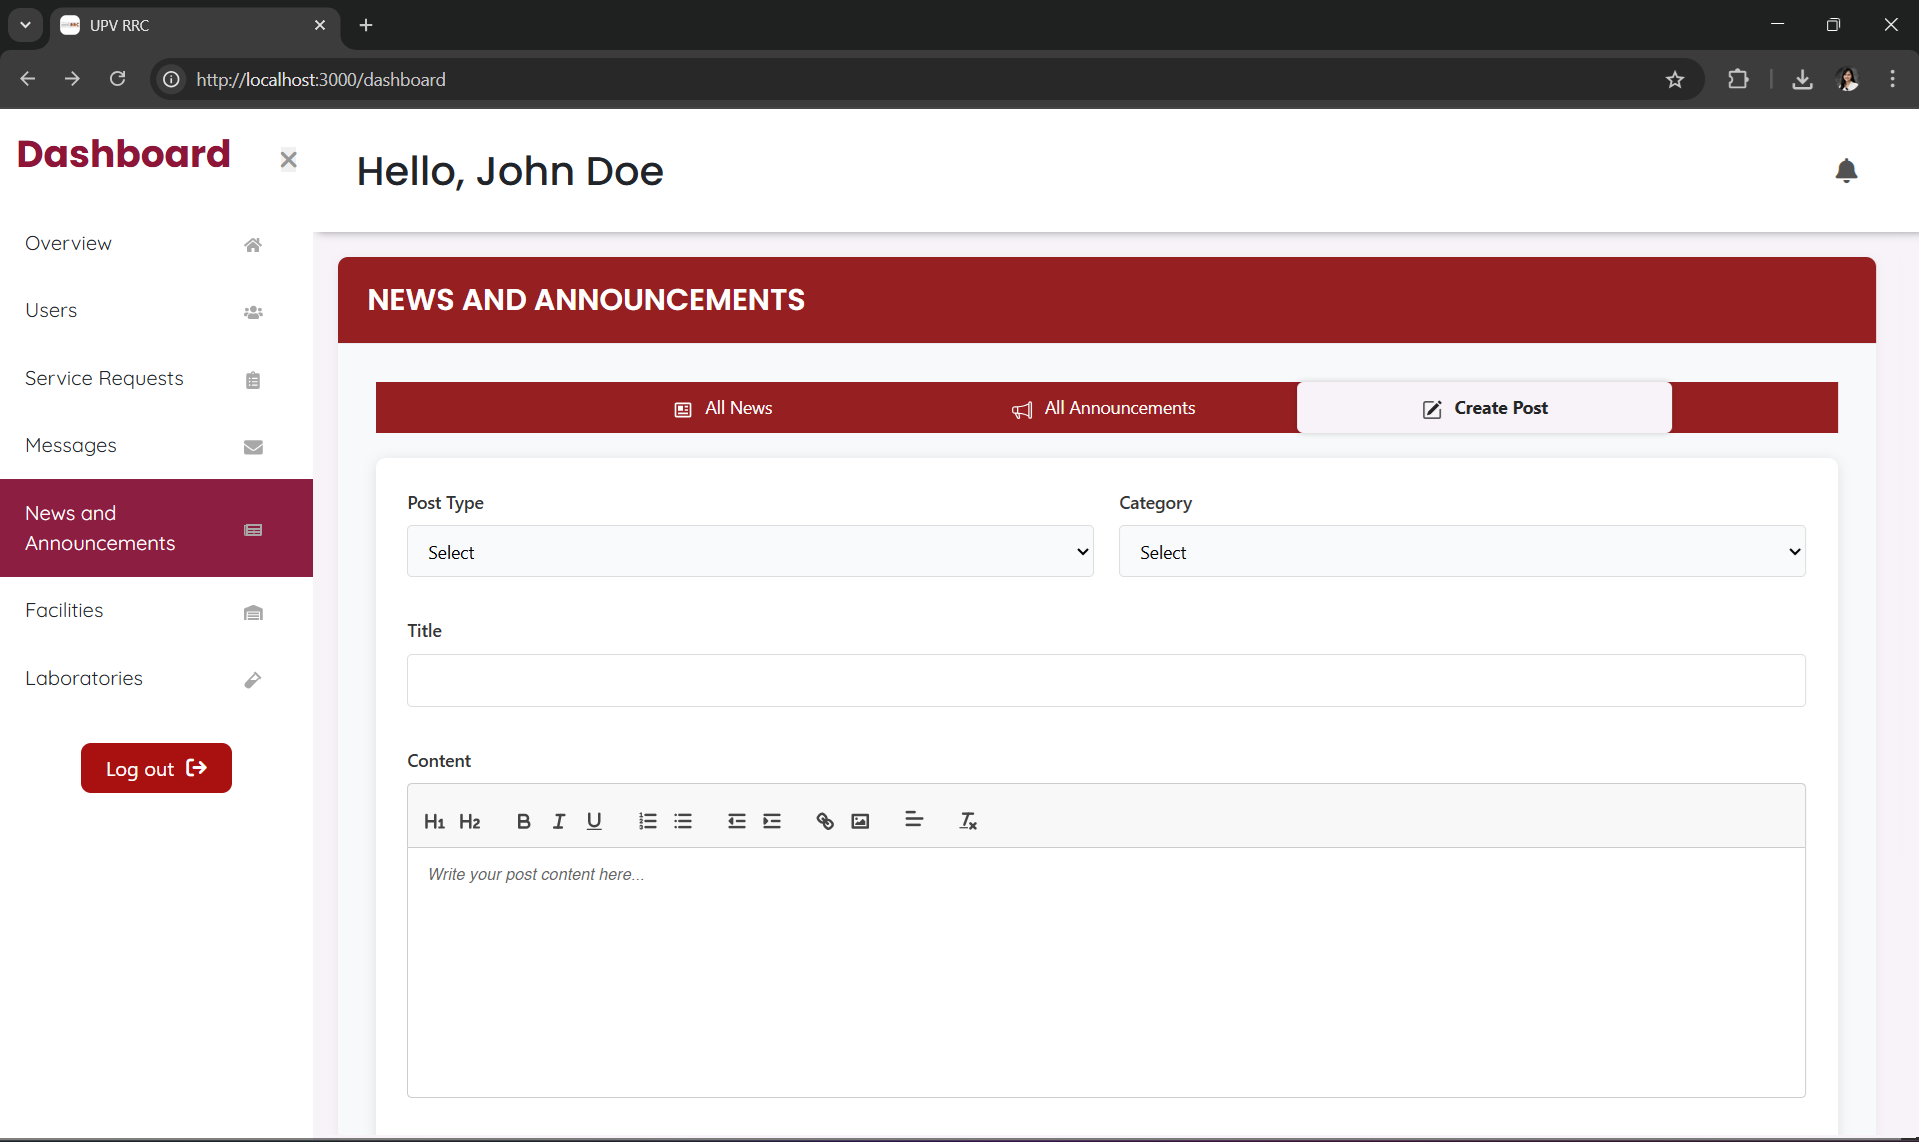
\includegraphics[width=0.8\textwidth]{news_section.png}
    \caption{Interface for creating News and Announcements}
    \label{fig:announcements}
\end{figure}

\newpage

\subsection{Data Management Module}

Data management module is responsible for handling all the data within the system. This includes information of clients, transaction histories, inventory of equipment, and tracking of facility schedules and availability. This modules ensures that accounts are properly maintained while also allowing the staff to easily keep record of everything that is related to the RRC's service requests. It also streamlines the assignment of resources to users, maintains an up-to-date inventory, and provides a comprehensive view of resources, allowing for efficient allocation and tracking. Moreover, it enables staff and clients alike to view real time availability of equipment and facility, further guaranteeing the smooth and efficient flow of  service requests. To ensure fairness and transparency, the system implements a first come, first serve basis for all service bookings. This policy was integrated based on the standard operating procedure of the RRC and ensures that all users have equal opportunity to access resources based on request order. When clients submit a service request, the system automatically logs the timestamp, and the requests are queued accordingly. This rule is clearly communicated to users through the interface, helping manage expectations and minimize booking conflicts.

\subsection{Chatbot}

The chatbot, named LIRA (Learning, Innovation, and Research Assistant), was successfully integrated into the TUKIB system. It appears as a floating button located at the bottom left corner of each page, allowing users to access assistance at any time.

Upon clicking the button, the chatbot initiates the conversation by presenting a welcome message, as shown in \figref{fig:chatbot_ui}. It then offers a set of predefined options to help users with possible queries. These include inquiries about laboratory services, frequently asked questions, and how to navigate the system. This setup reduces the workload on support staff and improves user satisfaction by providing immediate answers.

\begin{figure}[h]
	\centering
	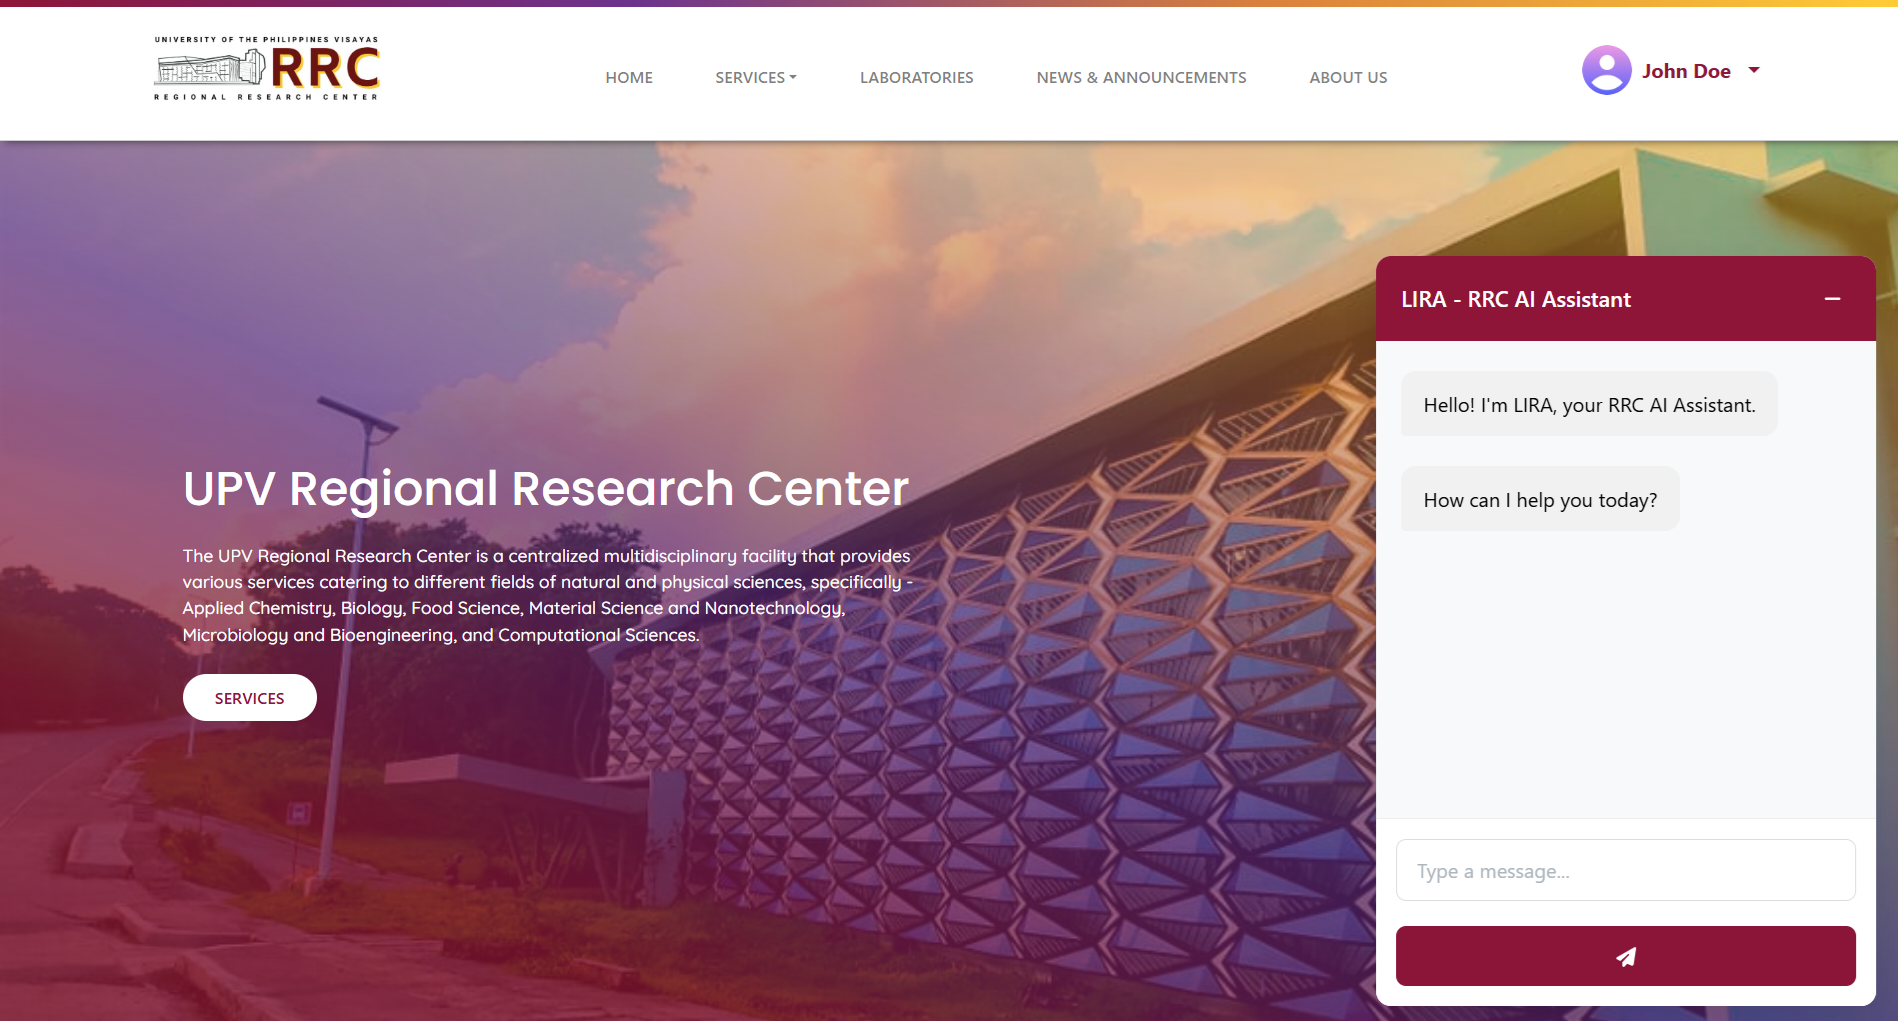
\includegraphics[width=0.8\textwidth]{chatbot_ui.png}
	\caption{Chatbot Interface}
	\label{fig:chatbot_ui}
\end{figure}

\subsection{Scope and Limitations of the Chatbot}

The chatbot was developed using the Rasa framework, which includes both a Natural Language Understanding (NLU) component and a dialogue management system. It is capable of handling various types of user intents such as greetings, general inquiries, and specific service-related questions.

In its current state, LIRA utilizes a set of predefined intents and responses based on a small, curated training dataset relevant to the Regional Research Center (RRC). The chatbot can perform initial consultation with new clients. Once the client's request is deemed feasible, the chatbot proceeds to collect the user’s details and using the provided details, the user's account will be created automatically by the system.

While LIRA improves user experience and reduces the workload on support staff, it has some limitations. It only supports the English language, which may hinder accessibility for non-English-speaking users. Additionally, it relies on a small, curated training dataset, limiting its ability to handle queries beyond its predefined scope.

\section{Data Privacy and Security Measures}

Ensuring the privacy and security of user data is a critical component of the TUKIB system. Several technical measures were implemented to protect user credentials, control access, and prepare for potential data loss scenarios.

\subsection{Password Encryption}

In order to ensure the security of user accounts, password hashing was implemented. This ensures that even if the database is compromised, plaintext passwords remain protected. The bcrypt algorithm was used due to its strength and resistance to brute-force attacks. Each password is hashed with a unique salt, which adds randomness and protects against rainbow table attacks.

During user registration, passwords are hashed before being stored in the database. During login, the hashed version of the input password is compared to the stored hash to authenticate users. This approach follows best practices in modern web security and ensures that sensitive credentials are never stored or transmitted in plain text.

\subsection{User Authentication and Authorization}

The system uses secure authentication and authorization mechanisms to manage user access and roles. These mechanisms include:

\begin{itemize}
	\item \textbf{Token-Based Authentication.} JSON Web Tokens (JWTs) are used to authenticate sessions securely. Tokens are issued upon successful login and used to verify user identity in subsequent interactions without exposing sensitive data.
	\item \textbf{Role-Based Access Control (RBAC).} Access to system functionalities is restricted based on user roles. For example, administrators, staff, and clients each have distinct permissions, reducing the risk of unauthorized actions.
	\item \textbf{Login Attempt Restrictions.} To mitigate brute-force attacks, the system enforces login attempt limits. After a specified number of failed login attempts, the account is temporarily locked, and further login attempts are blocked for a cooling-off period.
\end{itemize}

\subsection{Terms and Conditions}

To ensure transparency and user accountability, the TUKIB system includes a Terms and Conditions agreement that users must acknowledge before submitting a service request. This agreement outlines the responsibilities of both the users and the UPV Regional Research Center, including provisions on proper usage of the system, adherence to facility protocols, and consent to data processing.

In the service request form, a checkbox is provided requiring users to confirm that they have read and agreed to the Terms and Conditions before proceeding. A hyperlink to the full Terms and Conditions document is embedded directly in the form text for convenient access. This serves as an initial layer of compliance with the system’s data privacy and security policies.

\begin{figure}[h]
	\centering
	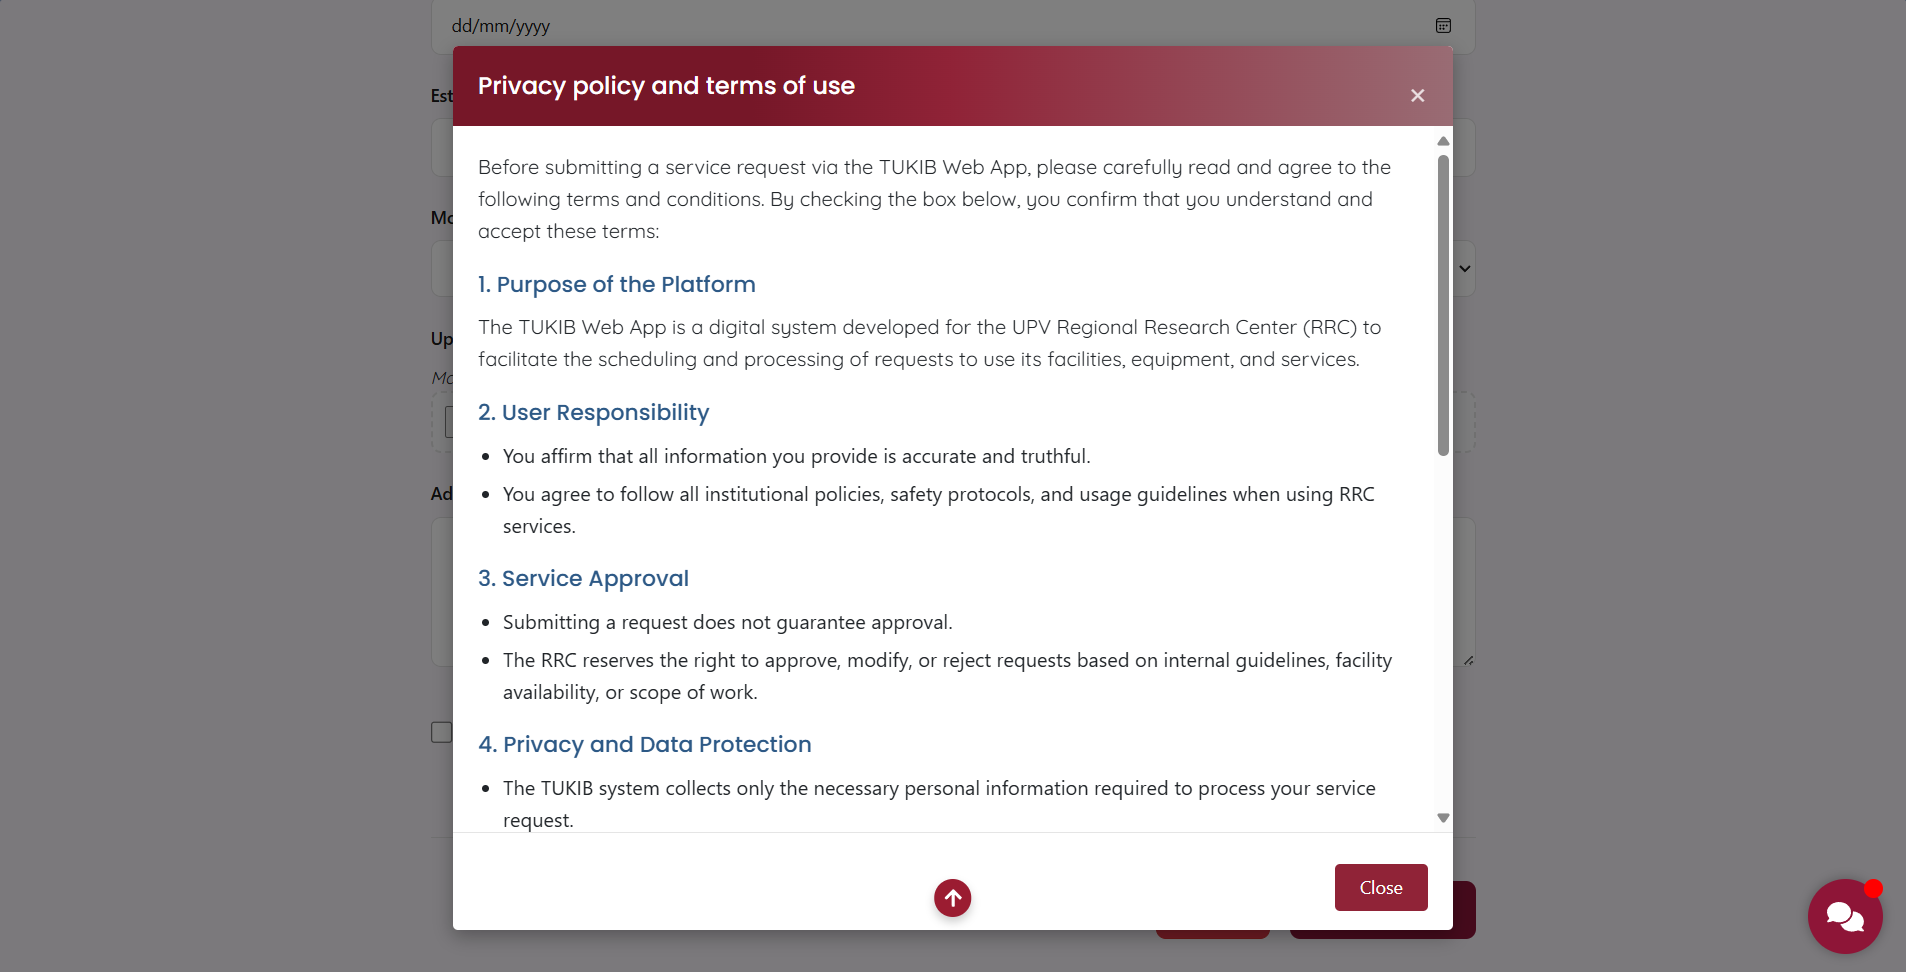
\includegraphics[width=0.8\textwidth]{terms.png}
	\caption{Terms and Conditions}
	\label{fig:terms}
\end{figure}

By requiring agreement to the Terms and Conditions before every service request, the system ensures that users are informed of the scope of their obligations and rights, particularly with regard to the handling of personal and research-related information. This step is crucial in promoting responsible usage and safeguarding sensitive data within the TUKIB platform.

\subsection{Backup and Recovery}

To safeguard against data loss caused by system failures, data breaches, or accidental deletions, automatic data archiving and backup mechanisms were implemented. The system is configured to perform regular backups of critical data in order to ensure that data can be restored in the event of an incident.

Backups are scheduled at defined intervals and stored securely, following best practices for data integrity and redundancy. These backups can be used to recover the system to a previously stable state, minimizing downtime and preventing permanent data loss. 

\section{Testing and System Evaluation}

The evaluation of the TUKIB system was conducted through multiple stages of testing, covering functionality, usability, performance, and chatbot effectiveness. Testing occurred both during development and after the completion of core features to ensure the system met its objectives and aligned with the operational needs of the UPV Regional 
Research Center (RRC).

\subsection{Functional Testing}

System testing was conducted alongside the development process to ensure the functionality of each module. Manual testing was performed for every feature, including form submissions, login, account creation, and data retrieval processes. Bugs and issues identified during this phase were addressed iteratively. To guide development, an RRC staff member was regularly consulted and provided necessary information and documents, offering critical feedback and clarifications on service workflows and operational requirements.

After implementing the system's core features, an internal review was conducted with RRC staff to evaluate whether the platform aligned with existing operations. This evaluation focused on how well the system supported service management and administrative tasks. Based on the feedback, several components—particularly those related to request processing and data workflows—were refined to better meet the institution’s needs.

\subsection{Usability Testing with End Users}

Usability testing was conducted to evaluate the system’s intuitiveness and user-friendliness from the perspectives of both staff and potential end users. During the internal review, RRC staff provided valuable feedback regarding interface improvements. Based on their suggestions, enhancements such as tooltips, clearer labels, and structured input elements— like dropdown menus and checkboxes— were implemented to simplify data entry and reduce user errors, especially in forms where the required information is predefined or known in advance.

Following this, external testing was conducted with potential end users—primarily students who represent the typical clientele of the RRC. Participants were asked to complete common tasks, such as submitting service requests and navigating through the dashboard. Feedback was gathered through observation and brief interviews, where users shared their overall experience, ease of navigation, perceived clarity of the interface, and suggestions for future improvements.

While the feedback indicated that users found the system easy to use, with a clear layout and generally responsive design, one notable issue was inconsistency in component behavior when the window was minimized or when the screen size differed from standard laptop or desktop dimensions. In these cases, some interface elements did not display or function optimally, affecting the overall responsiveness.

Despite this, features such as tooltips, clearly labeled buttons, and real-time feedback messages were highlighted as particularly helpful in guiding user interactions. These findings suggest that the system mostly meets its objective of providing an intuitive and user-friendly interface for both RRC staff and clients, while leaving room for improvements in adaptive design and overall intuitiveness.

\subsection{Performance Testing}

Performance testing was conducted to evaluate the system's responsiveness and stability. Due to resource and technical constraints, testing was limited to small-scale scenarios involving light usage conditions (e.g., one to two users on a local server setup). Key interactions—such as logging in, submitting forms, and using the chatbot—were tested for responsiveness and reliability. Cross-browser compatibility was also validated using popular browsers including Google Chrome, Mozilla Firefox, and Microsoft Edge to ensure consistent functionality across platforms.

\subsection{Chatbot Evaluation}

The chatbot component, LIRA, was tested for responsiveness and effectiveness in assisting users through a series of predefined test scenarios and real-user interactions. Testing involved inputting a variety of queries related to frequently asked questions and service inquiries to evaluate the chatbot’s ability to understand and respond appropriately. LIRA is built on a rule-based system using the Rasa framework, relying on a curated training dataset exclusively in English. Consequently, queries falling outside the predefined intents or those that were ambiguous could not be adequately addressed, resulting in generic or fallback responses. During testing, LIRA successfully handled many common questions but exhibited limitations when processing inputs containing proper names and numerical data such as phone numbers or dates. Additionally, the chatbot was case-sensitive, which affected its ability to interpret queries when capitalization varied. The English-only training data further restricted accessibility, limiting support for non-English-speaking users. These findings indicate areas for future improvement, particularly in expanding natural language understanding capabilities and enabling multilingual support of the chatbot.

\section{Methodological Constraints}

Although the Agile methodology offered flexibility during the development of TUKIB, several inherent disadvantages emerged throughout the development process. For instance, scheduling conflicts occasionally delayed feedback sessions and document requests, as stakeholders were sometimes unavailable due to other responsibilities. This resulted in uneven progress across modules— some were further refined, while others lagged due to postponed input. In certain cases, components were implemented differently than initially planned because of these limitations. Additionally, the focus on adaptability made long-term planning more difficult, and some documentation tasks were not prioritized in favor of rapid iteration.

These limitations did not critically hinder the overall development, but they highlight areas where future teams may benefit from more structured planning, improved stakeholder coordination, and clearer documentation protocols, especially when working on institutional systems like TUKIB.

\section{Summary of Results}

To summarize the results of the study, the checklist of system requirements, Table \ref{tab:requirements}, was updated to indicate whether each requirement for TUKIB has been implemented. As shown in the Table \ref{tab:summary_results}, all of the system requirements have been successfully accomplished, demonstrating that the core functionalities of TUKIB are in place. Moreover, based on the evaluation and feedback from testing, the final output of this paper is agreed to meet the requirements needed by the users, especially by the RRC staff. 

\begin{table}[ht]
	\centering
	\begin{tabular}{|p{10cm}|c|}
		\hline
		\textbf{Requirements/Modules} & \textbf{Accomplished (Y/N)} \\
		\hline
		\multicolumn{2}{|l|}{\textbf{Backend Requirements}} \\
		\hline
		Local Database & Y \\
		Automatic archiving & Y \\
		RESTful API & Y \\
		Role-based access control & Y \\
		Error handling, validation, \& logging & Y \\
		\hline
		\multicolumn{2}{|l|}{\textbf{Privacy Requirements}} \\
		\hline
		User password encryption & Y \\
		Session or token authentication & Y \\
		Restriction of unauthorized access & Y \\
		Log in attempts limit/Brute-force protection & Y \\
		\hline
		\multicolumn{2}{|l|}{\textbf{User Interface Requirements}} \\
		\hline
		Client interface & Y \\
		Admin Staff interface & Y \\
		University Researcher interface & Y \\
		TECD Staff interface & Y \\
		Director interface & Y \\
		\hline
		\multicolumn{2}{|l|}{\textbf{Functional Requirements}} \\
		\hline
		User registration and authentication & Y \\
		Request tracking and management & Y \\
		Feedback mechanism & Y \\
		Notification system & Y \\
		Calendar system & Y \\
		Chatbot for FAQs and initial consultation & Y \\
		End-to-end flow of service request process & Y \\
		\hline
		\multicolumn{2}{|l|}{\textbf{UI/UX Design Requirements}} \\
		\hline
		Responsive design & Y \\
		User-friendly navigation & Y \\
		Feedback/confirmation messages & Y \\
		\hline
	\end{tabular}
	\caption{System Requirements Checklist Result}
	\label{tab:summary_results}
\end{table}